\documentclass{IEEEtran}

\special{papersize=8.5in,11in}
\usepackage{amsmath}
\usepackage{amssymb}
\usepackage{mathptm}
\usepackage{url}
\usepackage{times}
\usepackage{graphicx,color}
\usepackage{CJKutf8}
\usepackage{multirow}
\usepackage{kotex}
\usepackage{gensymb}
%\usepackage{stfloats}


\setlength{\emergencystretch}{2em}
\setlength{\parindent}{0em}

\begin{document}

\title{Runtime Power Management for Extended Range of Battery Electric Vehicles}

\author{
Donkyu~Baek,~\IEEEmembership{Member,~IEEE,} 
and~Naehyuck~Chang,~\IEEEmembership{Fellow,~IEEE}

\thanks{Direct questions and comments about this article to Naehyuck Chang, Korea Advanced Institute of Science and Technology, 291, Daehak-ro, Yuseong-gu, Daejeon, Korea (e-mail: naehyuck@cad4x.kaist.ac.kr). This work is supported in part by NRF Grant 2015R1A2A1A09005694.}
}

\maketitle

\begin{abstract}
Installation of a large-capacity battery pack is a straightforward method to extend the range of battery-electric vehicles (BEV, or all-electric vehicles.) However, at the same time, a large-capacity battery pack not only occupies a big space but significantly increases the vehicle weight, which directly impacts on the  fuel economy and vehicle performance. This implies that increasing the battery capacity has an obvious limitation in extending the EV range. In this paper, we introduce a system-level framework that derives the minimum-energy velocity at each time instance (velocity planning) from the vehicle dynamics, electric powertrain characteristics, road slopes, payload, and consideration of regenerative braking. This work particularly takes into account driving time so that the resultant minimum-energy-velocity planning does not seriously slow down the vehicle. 

The resultant velocity planning achieves range extension with the existing electric powertrain. The major technical contributions of this paper compared with the previous work include i) practically applicable minimum-energy-velocity planning for production EVs from superb EV power model fidelity, ii) new performance metrics to consider both driving energy and driving time, i.e., energy-delay product, energy-square-delay product and energy-cubic-delay product that ensures both energy consumption and driving time, iii) comparative analysis of the minimum-energy-velocity planning between EV and internal combustion engine vehicles (ICEV), and iv) analysis of the model fidelity impact on the minimum-energy-velocity planning. The proposed method results in up to a 43.4\% extended range and a 20.6\% improvement of the energy-delay product compared with the best constant-velocity driving.
\end{abstract}

%%%%%%%%%%%%%%%%%%%%%%%%%%%%%%%%%%%%%%%%%%%%%
\begin{IEEEkeywords}
Electric vehicles, minimum-energy-velocity planning, driving range extension
\end{IEEEkeywords}
%%%%%%%%%%%%%%%%%%%%%%%%%%%%%%%%%%%%%%%%%%
\section{Introduction}
%%%%%%%%%%%%%%%%%%%%%%%%%%%%%%%%%%%%%%%%%%

Battery-electric vehicles (BEV) or all-electric vehicles are powered sorely by the battery and thus generally cause range anxiety for most EV owners because their fully-charged range is much shorter than that of internal combustion engine vehicles (ICEV.) Lack of charging facility and longer charging time make the anxiety stronger, which is comparable to vehicle breakdown.

Unfortunately, it is hard to achieve a longer range from further efficiency enhancement of the major electric powertrain components such as traction motors, power converters, batteries, and so on, because they already exhibit a high efficiency (90\% or higher), and thus the headroom for further enhancement is very narrow.

A straightforward way to extend the range is to install a larger-capacity battery. However, this method does not only cause a higher manufacturing cost but higher daily operating cost because it  directly increases the vehicle curb weight, which is inversely proportional to the fuel economy~\cite{Hong:ASPDAC16}. Carrying a large-capacity battery also makes the passenger compartment smaller. In addition, the increased weight also directly impacts on the performance of the vehicle. 
EVs should be equipped with a more powerful drivetrain to compensate the weight increase, which again makes EV consume more energy. 
EVs deploy a large portion of light materials such as aluminum and carbon fiber to compensate the heavy battery weight not to degrade the fuel economy and performance significantly~\cite{Chang:ICCAD14}. However, such a way also causes a significant manufacturing and repairing cost increase because light materials that ensure strength are generally very expensive and not repairable by sheeting. Such conventional ways to extend the EV range directly impacts on the cost of ownership.

This paper introduces a runtime power management to extend the range without increasing the cost of ownership. EV energy consumption is largely different by the cruising velocity, acceleration, weight, load slope, etc. \cite{Chang:ICCAD14}. The concept of low-energy vehicle driving comes to reduce $CO_2$ emissions from ICEV. Lower  $CO_2$ emission generally implies less fuel consumption~\cite{Seraens:thesis12}. 

However, low-energy ICEV driving results are not applicable to EVs due to significant differences 
between the engine  and electric  powertrain. An internal combustion engine with a transmission is a common ICEV powertrain structure while EV electric powertrain has an electric motor with a fixed ratio gearbox (a reducer.) A transmission is a mandatory component of ICEVs as the engine torque and power are distinct convex functions of the engine RPM (revolutions per minute.) On the other hand, electric motors have a flat torque from zero RPM to the base (rated) RPM. Such advantage enables passenger vehicles not to mandate a transmission as long as there is not significant variation in the payload like a heavy-duty trucks and buses. A higher motor RPM over the base speed is achieved by the use of field weakening, and a single reduction ratio gear box can exhibit a fast enough top velocity. Regenerative braking is another advantage of EVs, which fundamentally changes the vehicle power consumption when it decelerates.

In this paper, we derive the minimum-energy velocity for a given EV and demonstrate its fundamental difference between that of ICEV. 
We derive an analytical EV power model with a scale of production EVs such as Chevrolet  Bolt. We introduce new performance metrics for EV, energy-delay product, energy-square-delay product and energy-cubic-delay product, which demonstrates a practically applicable minimum-energy-velocity planning. The proposed method results in up to a 43.4\% extended driving range without increasing battery capacity, and a 20.6\% improvement of the energy-delay product compared with the best constant-velocity driving. 

%%%%%%%%%%%%%%%%%%%%%%%%%%%%%%%%%%%%%%%%%%
\section{Related work} \label{sec:related work}
%%%%%%%%%%%%%%%%%%%%%%%%%%%%%%%%%%%%%%%%%%
  
The minimum-energy-velocity planning is proposed for ICEVS to assists drivers in order to save fuel consumption and reduce emissions~\cite{Seraens:thesis12, Kamal:TITS11, Ozatay:TITS14, Dovgana:ASC14, Ozatay:IFAC14, Khayyam:ESA12}.  
The fuel consumption model is a polynomial form based on a general vehicle dynamics model and takes into account the transmission shift position. 

There have been low-energy driving research for EVs as well, but previous research relies on the  vehicle dynamics models such as rolling resistance, gradient resistance, aerodynamic resistance, and so forth~\cite{Yan:NAPS14}, which ignores loss of energy transformation from electricity to mechanical energy. Such simplification makes it impossible to count on the powertrain efficiency at all, regardless of ICEV or EV. 

It has been reported that even EV power models that consider the motor loss~\cite{Lin:ICCA14, Wu:ITS15, Dib:IVPPC11} can hardly reproduce correct EV drivetrain power consumption~\cite{Hong:ASPDAC16}. This paper  demonstrates how incorrect EV power model can mislead the low-energy velocity planning in Section~\ref{sec:energy consumption}. 

There have been previous practices that demonstrate how EVs should change the vehicle velocity to reduce energy consumption under  a given road and traffic conditions. Such work commonly formulates an offline optimization problem and uses a dynamic programming (DP) to derive the globally optimal solution~\cite{Lin:ICCA14, Dib:IVPPC11, Dib:OGST12, Mensing:TR13}. However, once again, such work usually uses the vehicle dynamics model for the EV power model. It borrows the parameters from commercial vehicles such as the vehicle curb weight, aerodynamic resistance from the vehicle specifications and the rolling resistance from the tire specifications~\cite{Lin:ICCA14}. 

An empirical modeling has a potential to achieve more accurate power model  of a particular target EV. Related work fabricates a custom EV, collects the GPS tracking, battery voltage and battery current and constructs an EV power consumption model with several parameters~\cite{Dib:IVPPC11}. However, this power model still has important parameters missing that significantly affect the model fidelity such as friction loss, iron loss and windage loss in the motor, loss in the drivetrain and regenerative braking. Inaccurate EV power consumption model misleads the minimum-energy-velocity planning. A more recent work fabricates a low-speed custom EV and derived an accurate power model. The power model reflects various EV-specific factors including regenerative braking and even for drivetrain loss by regression analysis of large amount of driving data. However, the power model is limited to low-speed EVs and hard to accommodate production EVs~\cite{Hong:ASPDAC16}. 

Some work attempts to accommodate more realistic driving conditions such as traffic signals and stop signs. However, the results are lack of practicality due to the assumption of a constant road slope and a constant cruising velocity with highly simplified EV power models~\cite{Yan:NAPS14, Dib:CEP14, Wu:ITS15}. 

%%%%%%%%%%%%%%%%%%%%%%
%Related work
We recently see a new initiative that attempts to reduce energy consumption of cyber-physical systems using application-aware cross-layer management. Such approaches apply algorithms, tools and methodologies relevant to design automation and embedded low-power systems~\cite{Seshia:TCAD17}. 
% Energy management 
Just naming several for instance, energy management for EV also considers drivers' behaviors and related EV power consumption to extend range~\cite{Vatanparvar:TSG18,Vatanparvar:TODAES17}.
% EV battery pack 
Electric vehicle battery packs consist of a large number of battery cells, and it is crucial to optimize the battery pack architectures in terms of capacity, cost and reliability~\cite{Wu:TCAD13,Shaheer:RTCSA17}. 
Electric vehicle battery management systems must be able to accommodate multi-power sources, provide a good scalability, and mitigate cell-to-cell variability~\cite{Shin:TCAD15}.
% Non-propulsion power
Electric vehicles consume a non-negligible amount of battery energy for non-driving power components. Related study tries to optimize energy for heating, ventilation and air conditioning (HVAC) systems equipped in electric vehicles~\cite{Zhao:ICCAD15,Vatanparvar:TECS18}. 
% Energy 
A renewable energy aware pricing scheme minimizes both the community-wide electricity bill and individual electricity bill~\cite{Liu:TPDS17}.
% HESS
A hybrid energy storage systems improve efficiency and lifetime without significant increase of the cost~\cite{Xie:TCAD13, Kim:JPS14}. 
%%%%%%%%%%%%%%%%%%%%%%




%%%%%%%%%%%%%%%%%%%%%%%%%%%%%%%%%%%%%%%%%%
\section{Vehicle Power and Energy Consumption Analysis} \label{sec:energy consumption}
%%%%%%%%%%%%%%%%%%%%%%%%%%%%%%%%%%%%%%%%%%

%%%%%%%%%%%%%%%%%%%%%%%%%%%%%%%%%%%%%%%%%%
\subsection{The minimum-energy-cruising velocity} \label{subsec:opt-cruising}

A commonly used vehicle power consumption model is from the vehicle dynamics equation~(\ref{eq:dynamics_model}). This model considers the traction force only assuming a 100\% efficiency of the powertrain (engines, electric motors or both.) Therefore, this model is applicable to any sort of vehicles but not able to explain EV-specific power consumption.
%
\begin{equation}  \label{eq:dynamics_model} %equation 1
\begin{split}
P_{trac}	&= F \frac{ds}{dt} = Fv= (F_{R} + F_{G} + F_{I} + F_{A}) v \\
F_{R} \propto C_{rr}W,~F_{G} &\propto Wsin\theta,~F_{I} \propto ma,~\text{and}~F_{A} \propto \frac{1}{2} \rho C_d Av^2 \\
P_{trac} &\approx (\alpha  + \beta sin\theta + \gamma a + \delta v^2)mv
\end{split}
\end{equation}
where $F_R$, $F_G$, $F_I$, $F_A$, and $F_B$ denote the rolling resistance, gradient resistance, inertia resistance, aerodynamic resistance, and brake force provided by hydraulic brakes, respectively~\cite{Park:DAC13}. The coefficients $\alpha$, $\beta$, $\gamma$, and $\delta$ correspond to the rolling resistance, gradient resistance, inertia resistance, and aerodynamic resistance, respectively.

The actual power consumption evaluation of ICEV, i.e., fuel consumption rate, should take into account the powertrain efficiency. A simplified model of ICEV fuel consumption in~\cite{Kamal:TITS11} is written as follows:
%
\begin{equation} \label{eq:power_ICEV} %equation 2
P_{ICEV} = \frac{P_{trac} + P_{start}}{\eta_{ICEV}} 
\end{equation}
where $P_{start}$ is power consumption of the engine during idling. The engine efficiency, $\eta_{ICEV}$, is determined by the gear ratio, engine speed and engine torque. The gear ratio generally dynamically changes by transmission shift. The engine efficiency is generally not simple enough to explain by analytic functions and often described as efficiency maps~\cite{Kamal:TITS11}.

Adding a traction motor power model in (\ref{eq:power_ICEV}) makes (\ref{eq:dynamics_model}) and (\ref{eq:power_ICEV}) reflect more realistic EV power consumption characteristics. 
%
\begin{equation} \label{eq:motorloss_model} %equation 3
P_{EV} = \frac{P_{trac}}{\eta_{EV}}
\end{equation}
\begin{equation}
\eta_{EV} = \frac{P_{trac}}{{P_{trac} + k_c T^2 + k_i \omega + k_w \omega^3 + C}}\nonumber 
\end{equation}
where $k_c$, $T$, $k_i$, $\omega$, $k_w$, $C$ represent a copper loss coefficient, a motor torque, a coefficient by iron and friction loss, an angular speed, a windage coefficient, and constant loss, respectively~\cite{Hong:ASPDAC16}.

EVs mostly use regenerative braking during deceleration, which converts kinetic energy to electric energy except low-cost golf carts. The harvested energy from regenerative braking is closely related to the electromagnetic flux inside of the motor, and the flux is proportional to the motor RPM. The regenerative braking model of an EV can be  simplified as (\ref{eq:regen_model}) 
%
\begin{equation}\label{eq:regen_model} 
P_{regen} = \epsilon T v + \zeta
\end{equation}  %equation 4
%
where $\epsilon$ and $\zeta$ are regenerative braking coefficients.

The power consumption model (\ref{eq:motorloss_model}) is commonly used in various analytical EV power managements~\cite{Dib:IVPPC11, Dib:CEP14, Wu:TR15}. However, there are still considerable sources of power loss from  the drivetrain. To make a long story short, (\ref{eq:dynamics_model}) -- (\ref{eq:motorloss_model}) do not accurately explain EV-specific power consumption in various driving conditions according to our intensive measurement with real EVs. 

In this paper, therefore, we borrow an EV-specific power ($EV^*$) modeling method considering the loss in EV drivetrain using a multivariable regression method from the measured power data and achieve a polynomial fitting~\cite{Hong:ASPDAC16}. However, we should not directly use this power model because the model covers only low-speed EVs, i.e., slower than 35 km/h. Thus, we derive our own model coefficients in this paper.
%
\begin{equation} \label{eq:EV_specific_model} %equation 5
P_{EV^*} = \frac{P_{trac}}{\eta_{EV^*}}
\end{equation} 
\begin{equation}
\eta_{EV^*} = \frac{P_{trac}}{{P_{trac} + C_0 + C_1 v + C_2 v^2 + C_3 T^2}}\nonumber
\end{equation}	
where $C_0$, $C_1$, $C_2$, and $C_3$ mean coefficients for constant loss, iron and friction losses, drivetrain loss, and copper loss, respectively. Even if (\ref{eq:EV_specific_model}) has the same form as (\ref{eq:motorloss_model}), the actual coefficients become different if it reflects the characteristics of electric powertrain. 

\begin{figure*}	%Figure 1.
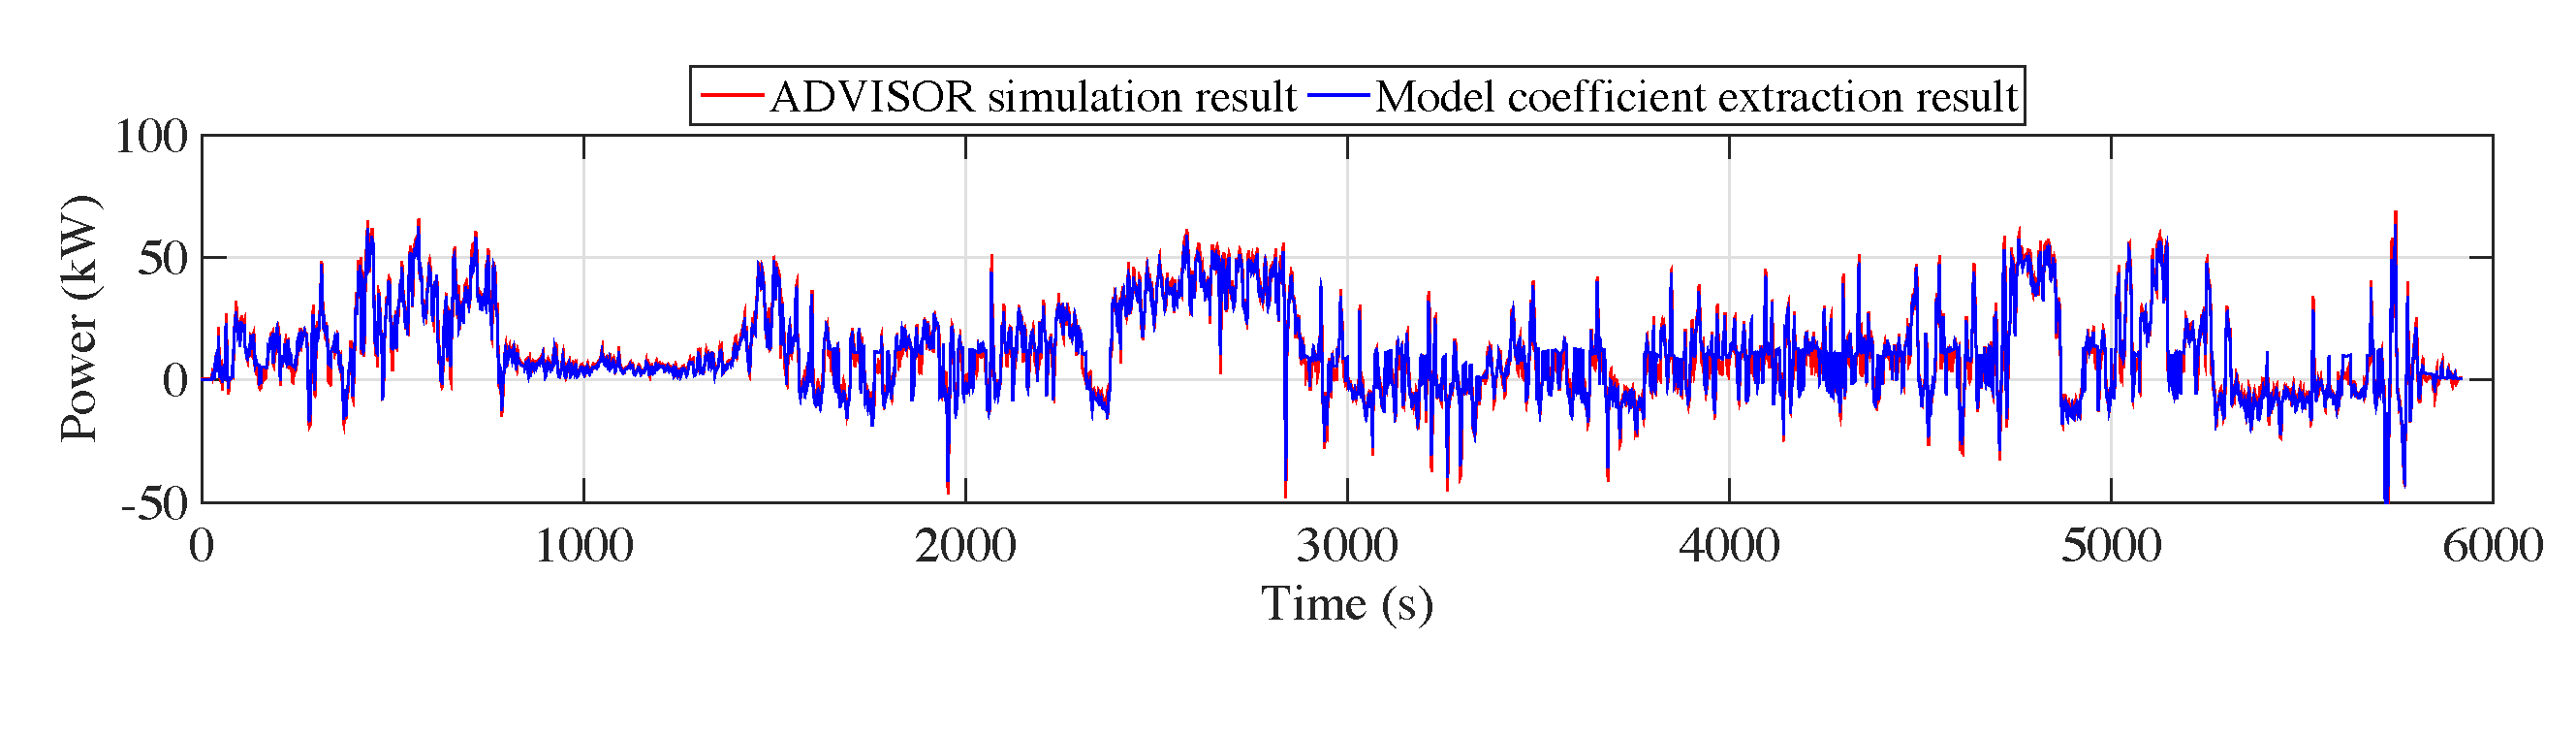
\includegraphics[width=1.0\hsize]{Figures/ADVISOR_model_validation_result.pdf}
\caption{Validation of the model coefficient extraction.}
\label{fig:ADVISOR_model_validation}
\end{figure*} 

ADVISOR is a vehicle simulator that takes into account various factors of vehicles including engines, electric traction motors, types of drivetrains, shape of chassis, etc.~\cite{Markel:JPS02}. ADVISOR is a sort of a fast vehicle simulator as it simulates a 700 second vehicle driving in one second. DP is commonly used to derive the energy-optimal velocity planning of vehicles~\cite{Lin:ICCA14,Dib:IVPPC11,Hellstrom:CEP09}. The DP optimization repeatedly computes the vehicle energy in each distance, velocity and acceleration step, and thus it is not proper to run ADVISOR in the inner loop of the DP optimization. For instance, it takes 15 minutes of computation to derive a 10 minute driving velocity planning profile with a 30-step velocity resolution. This is absolutely not acceptable for online recomputation that can be caused by unexpected interrupts while driving. So, instead of using ADVISOR for the speed optimization, we use ADVISOR for the model coefficient extraction. In other words, we use the same form of polynomial as~\eqref{eq:EV_specific_model} but derive the coefficients by running ADVISOR.

We choose Chevrolet Bolt (1,616 kg curb weight) for the target vehicle, but our method does not restrict a particular type of vehicles. The top speed of Chevrolet Bolt is 150 km/h. It is capable of achieving a 6.5 second 0--100 km/h time with a 150 kW electric permanent magnet motor~\cite{GM_Bolt:official}. Chevrolet Bolt is equipped with a 350 V and 57.4 kWh Lithium-ion battery pack with 96-series and 3-parallel of 3.65 V cells~\cite{GM_Bolt:spec}. 

We first implement a Chevrolet Bolt power model based on the vehicle specifications and reports for the Chevrolet Bolt performance and range at various constant velocities~\cite{GM_Bolt:range25mph,GM_Bolt:range65mph,GM_Bolt:range75mph,GM_Bolt:range93mph}. We extract the model coefficients of~\eqref{eq:EV_specific_model} by running ADVISOR. The model coefficient extraction result shows as in Figure~\ref{fig:ADVISOR_model_validation}. The normalized root-mean-square deviation is 5.1\%. Table \ref{table:Coeff_Bolt} summarizes the model coefficients of (\ref{eq:EV_specific_model}) for Chevrolet Bolt. 

\begin{table}
\caption{Model coefficients for Chevrolet Bolt.}
\label{table:Coeff_Bolt}
\centering
\begin{tabular}{|c|c|c|c|c|c|}  \hline
$\alpha$	&0.06		&$\beta$	&9.5549	&$\gamma$	&1.0013	\\ \hline
$\delta$	&0.00012 		&$C_0$	&1000 	&$C_1$		&10.588	\\ \hline
$C_2$	&8.11		&$C_3$	&0.00032	&$\epsilon$	&0.6633	\\ \hline
$\zeta$	&5813.6		\\ \cline{1-2}
\end{tabular}
\end{table}

%%%%%%%%%%%%%%%%%%%%%%%%%%%%%%%%%%%%%%%%%%
\subsection{Energy consumption comparison between ICEV and EV} \label{subsec:comparison}

We compare power consumption behavior of EV and ICEV in this section. As most previous fuel economy analysis work is done by energy (fuel) consumption, we compare energy consumption instead of power consumption for easy comparison. 

\begin{figure}	%Figure 2.
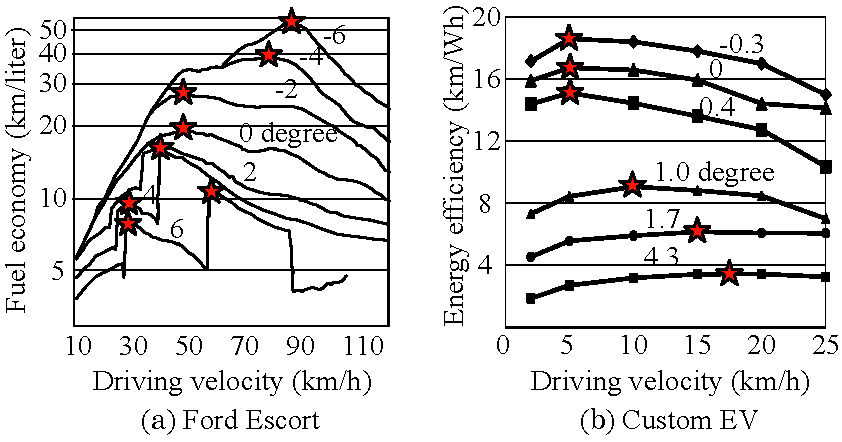
\includegraphics[width=1.0\hsize]{Figures/ICEV_EV_consumption.pdf}
\caption{(a) Fuel economy of a Ford Escort~\cite{Hooker:TR88} and (b) energy consumption of a custom EV~\cite{Chang:ICCAD14} on various road slopes and vehicle velocities.}
\label{fig:ICEV_EV_consumption}
\end{figure} 

Figure~\ref{fig:ICEV_EV_consumption}(a) shows the fuel economy (range with a liter of fuel energy) versus ICEV velocity on various road slopes~\cite{Hooker:TR88}. Red stars denote  the minimum-energy velocity by the average road slope. The minimum-energy velocity is reduced as the road slope increases. For example, the vehicle has the highest fuel economy at 90 km/h on  a $-6$ degree road slope and 40 km/h on a 2 degree road slope.  Fuel economy on a downhill (negative road slope) is not meaningful due to ``fuel cut" of modern ICEVs. Compared with the flat road (zero degree), we see the fuel economy drops if the road slope is steeper than 2 degree due to gear shift down.

Figure~\ref{fig:ICEV_EV_consumption} demonstrates s a very interesting EV-specific energy behavior such that the minimum-energy velocity increases as the road slope increases. Such energy behavior is completely opposite to that of ICEV. 
%
The efficiency maps of an  engine and an electric motor (Figure~\ref{fig:efficiency_map}) show that the motor exhibits  the maximum torque over the wide range of RPM while the engine exhibits the maximum fuel efficiency only at near 2,000 RPM. Therefore, an engine should be incorporated with a transmission that makes it possible to run the engine at close to the most efficient region, independent to the vehicle velocity. The required engine torque multiplied by the gear ratio (determined by the transmission shift position) also changes by the vehicle gradient resistance (road slope.) The optimal  transmission shift position and the minimum-energy velocity are thus determined by the road slope.

On the other hand, a fixed ratio gearbox is generally sufficient for EV since electric motors obtain the maximum torque over the wide range of RPM. The minimum-energy velocity is solely determined by the motor efficiency, which is a function of the torque and RPM. 
%
\begin{align}
E_{EV^*} 	&= \int_{T_{drive}} P_{EV^*}(v_{const})~dt \nonumber\\
		&= \frac{P_{trac}}{\eta_{EV}(T, \omega)} \int_{T_{drive}} dt  \nonumber\\
		&= \frac{F_{trac} \times v_{const}}{\eta_{EV}(T, \omega)} T_{drive}
		= \frac{F_{trac} \times D_{drive}}{\eta_{EV}(T, \omega)} \nonumber
\end{align}
where $T_{drive}$, $V_{const}$ and $D_{drive}$ denote the driving time, constant velocity and driving distance, respectively. Energy consumption, $E_{EV}$, with a constant velocity on a given road slope is sorely determined by the motor efficiency, $\eta_{EV}$. 

As the road slope becomes higher, the motor RPM would better be increased to achieve a higher motor efficiency according to the motor efficiency map in Figure~\ref{fig:efficiency_map}(b). The minimum-energy velocity of EV increases as the RPM increases because of the fixed single ratio gearbox. It is not possible to derive the minimum-energy velocity for EVs by applying  the minimum-energy velocity for ICEVs because of such discrepancies in the powertrains.

\begin{figure}	%Figure 3.
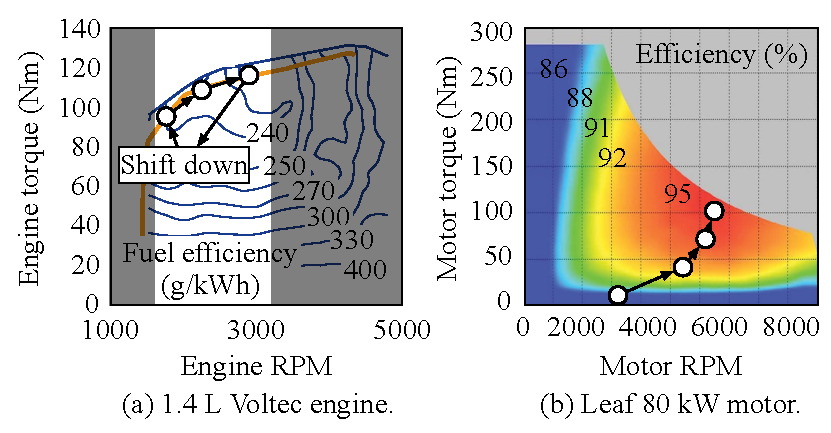
\includegraphics[width=1.0\hsize]{Figures/efficiency_maps.pdf}
\caption{Efficiency maps of (a) the GM 1.4 liter Voltec engine and (b) the Nissan Leaf 80 kW electric motor.}
\label{fig:efficiency_map}
\end{figure} 

%%%%%%%%%%%%%%%%%%%%%%%%%%%%%%%%%%%%%%%%%%
\section{Framework for Minimum-Energy-Velocity Planning} \label{sec:framework}
%%%%%%%%%%%%%%%%%%%%%%%%%%%%%%%%%%%%%%%%%%

%%%%%%%%%%%%%%%%%%%%%%%%%%%%%%%%%%%%%%%%%%
\subsection{Constant-velocity driving} \label{subsec:constant drive}

\begin{figure} %Figure 4
\centering
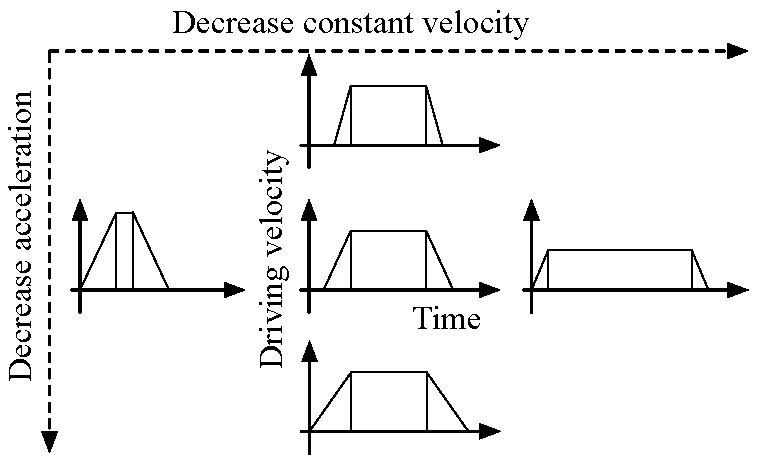
\includegraphics[width=0.9\hsize]{Figures/const_vel_drive_problem.pdf}
\caption{Various constant velocity and acceleration cases for the same distance.}
\label{fig:const_vel_drive_problem}
\end{figure} 

A constant-velocity driving is not always impractical and actually  useful to insure a steady  traffic flow and safety. Drivers often drive their vehicles up to the speed limit or slightly over the speed limit following the flow mainly aiming at shortest possible driving time. However, when it comes to the minimum-energy-velocity planning, a constant-velocity driving should use the minimum-energy velocity. 

We demonstrate how the cruising velocity, acceleration and deceleration affect EV energy consumption. We perform a design space exploration (DSE) for all feasible vehicle velocities and the acceleration pairs. We obtain the minimum-energy velocity and the initial and final acceleration for a given driving distance  as shown in Figure~\ref{fig:const_vel_drive_problem}. The results of DSE on a flat road (0 degree road slope) and a 4 degree road slope are shown in Figures~\ref{fig:DSE}(a) and \ref{fig:DSE}(b), respectively. The point at the minimum energy consumption per distance (Wh/km) represents the best constant-velocity driving. Surprisingly, the same distance driving requires significantly different amount of energy by the cruising velocity and acceleration as shown in Figure~\ref{fig:const_vel_drive_problem}. The energy consumption by the cruising velocity and acceleration pairs also completely changes by the road slopes. These examples indeed show a great potential to save energy consumption of EV with the proposed minimum-energy-velocity planning.

\begin{figure} %Figure 5
\centering
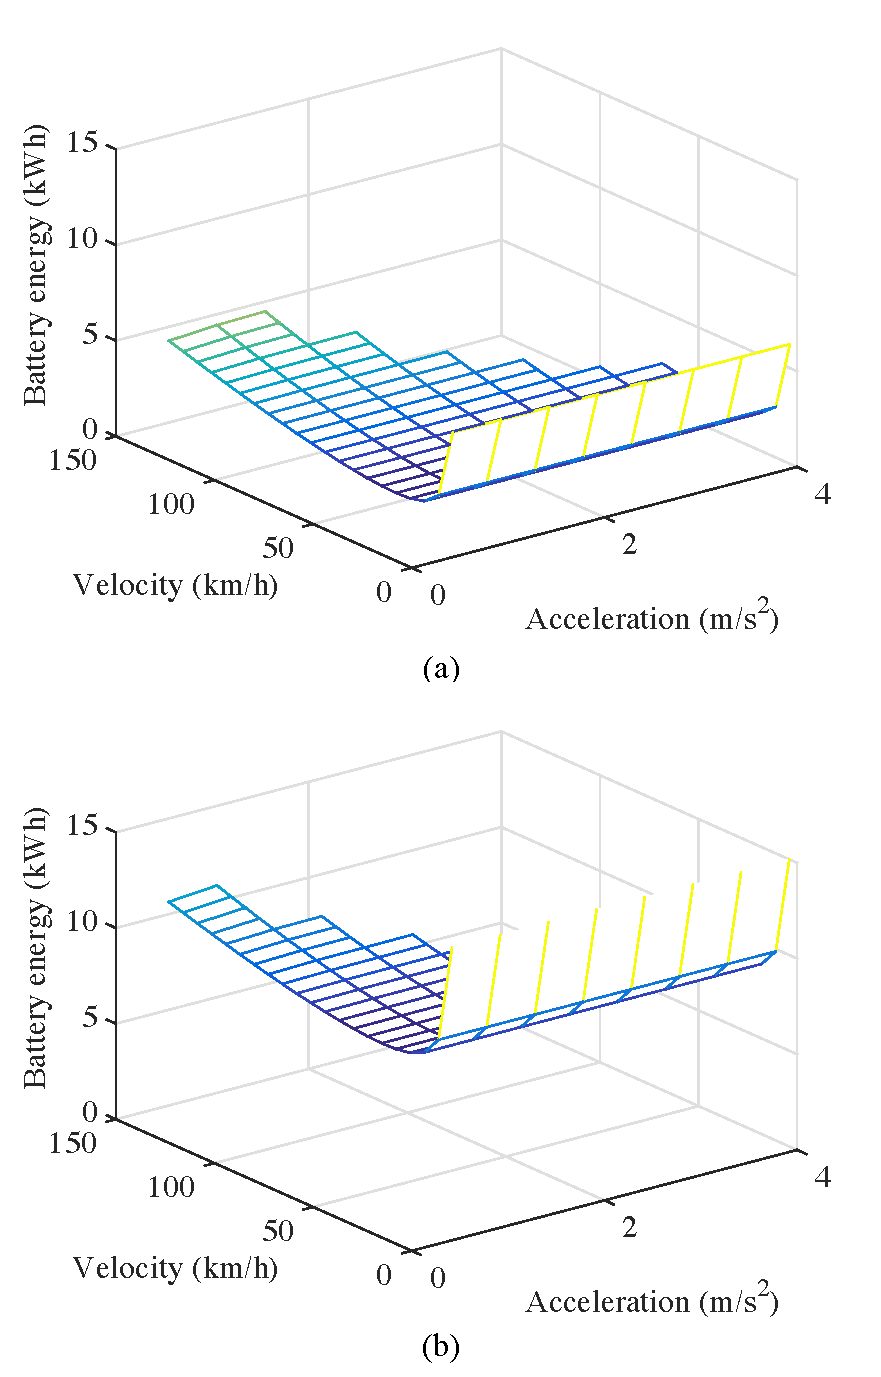
\includegraphics[width=0.95\hsize]{Figures/Design_space_exploration.pdf}
\caption{DSE of the best constant-velocity driving on (a) a 0 road slope and (b) a 4 road slope.}
\label{fig:DSE}
\end{figure} 

%%%%%%%%%%%%%%%%%%%%%%%%%%%%%%%%%%%%%%%%%%
\subsection{The minimum-energy-velocity planning} \label{subsec:variable drive}

\begin{table} 
\caption{Road benchmarks.}
\centering
\label{table:road_bench}
\begin{tabular}{|c|c|c|c|}  \hline
\multirow{2}{*}{Road index (\#)}
			&\multicolumn{3}{|c|}{Road slope (degree)}  \\ \cline{2-4}
			&Minimum 	&Maximum 	&Average \\ \hline
1			&-3.0 		&3.0 			&0.0 	  	\\ \hline
2			&-4.6 		&6.7 			&0.5 		\\ \hline
3			&-5.1 		&5.1 			&0.0 		\\ \hline
4			&0.0 			&3.0 			&0.8		\\ \hline
5			&0.0 			&7.6 			&3.0 		\\ \hline

\end{tabular}
\end{table}

\begin{figure} [h]%Figure 6
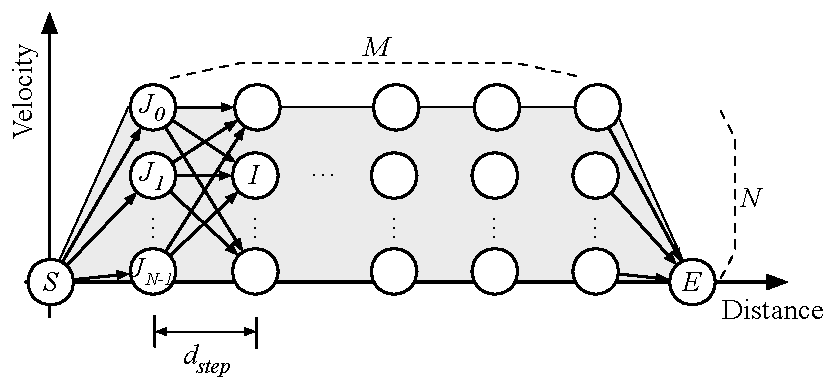
\includegraphics[width=1.0\hsize]{Figures/Opt_drive_problem.pdf}
\caption{Problem formulation to explore the minimum-energy-velocity planning.}
\label{fig:Opt_drive_problem}
\end{figure}

This subsection introduces a generalized minimum-energy-velocity planning for EV  on a road with variable slopes. We construct a DP to find the minimum-energy-velocity over distance. The DP obtains a set of the minimum-energy-velocity values for every distance step. In Figure~\ref{fig:Opt_drive_problem}, the X-axis and Y-axes denote the driving distance from the starting point and the driving velocity, respectively. Each node indicates the driving velocity at a given distance, and an edge between two nodes implies acceleration or deceleration during the distance step ($d_{step}$.) The maximum velocity is $v_{max}$, and the velocity step between two nodes at the same distance is $v_{step}$. The number of the nodes in each distance step is $N = v_{max} / v_{step}$, and the number of edges for a distance step is $N^2$. One node has $N$ edges going to the next distance, and a node receives $N$ edges. For example, a set of previous nodes, $J_0, J_1, \cdots, J_{N-1}$, goes to the next distance node (Node $I$.) As total number of steps to the endpoint is $M = (driving~distance) / d_{step}$, total number of nodes and edges are $MN$ and $MN^2$, respectively. There are only two nodes indicating 0 $m/s$ at the starting point (Node $S$) and endpoint (Node $E$.) A solution of the problem is a sequence of a node selection every distance step from Node $S$ to Node $E$. The objective and the constraints are defined as
%
\begin{align} %Equation 6
Min ~& \sum_{d=1}^{M}\sum_{v=1}^{N}\{\Delta t \frac{x(d,v)P_{d,v} + x(d-1,v)P_{d-1,v}}{2}\} \label{eq:objective}\\
Subject~to ~& \sum_{v=1}^{N}x(d,v) = 1~~where~~x(d,v) = \{0, 1\} ~~~\forall d, v \nonumber
\end{align}
%
where $\Delta t$ is a time to pass a distance step with a given velocity $v$, $d$ is a distance from the starting point and $P_{d,v}$ is a power consumption for a node with $d$ and $v$. $\Delta t$ varies by the driving velocity and acceleration. We set $x(d,v)=1$ once we accept the node at a distance $d$ and the velocity $v$.  We assume the EV should not drive too slow just for energy saving in order not to bother traffic (10 km/h). We also enforce the minimum acceleration as $ 0.4 m/s^2$ without loss of generality. 

\begin{figure*}	%Figure 7
\centering
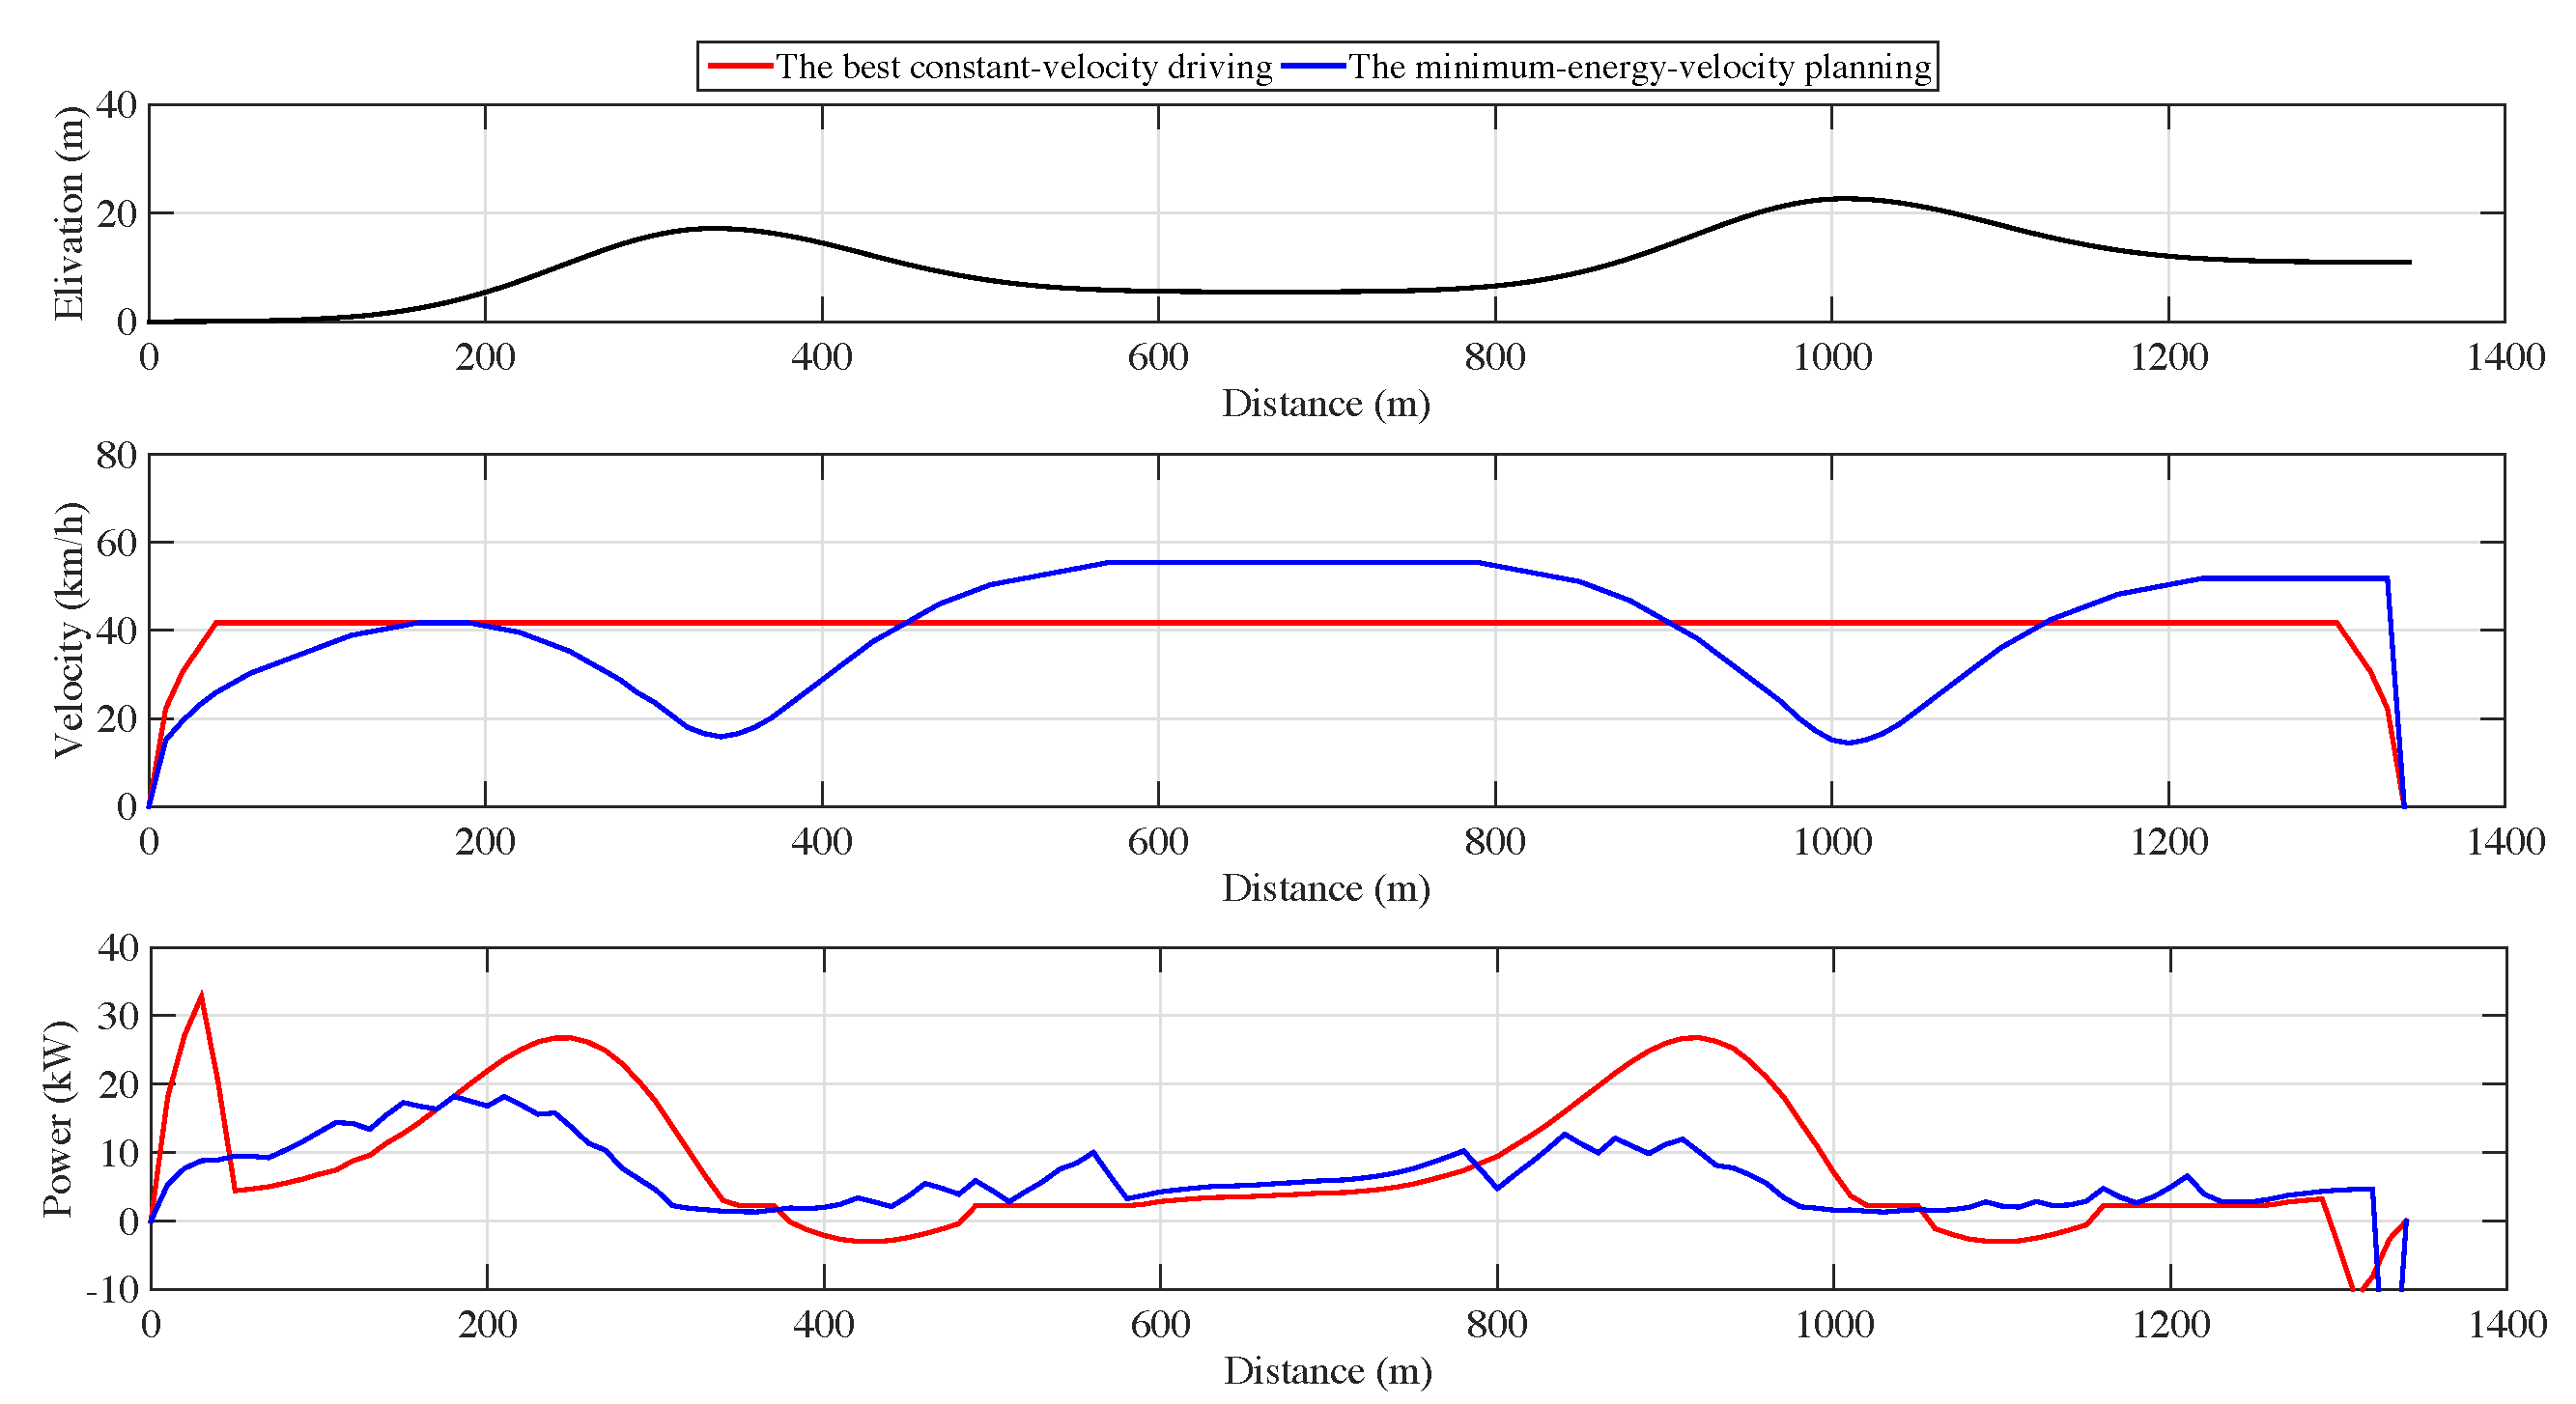
\includegraphics[width=1.0\hsize]{Figures/velocity_planning_road_Z.pdf}
\caption{Results of the minimum-energy-velocity planning.}
\label{fig:no_deadline_trace}
\end{figure*} 

We compare the simulation results between the best constant-velocity driving and minimum-energy-velocity planning. Figure~\ref{fig:no_deadline_trace}(a) shows the benchmark road including from $-4.5$ to 6.7 degree road slopes. From Figure~\ref{fig:no_deadline_trace}(b) to Figure~\ref{fig:no_deadline_trace}(d) show the minimum-energy-velocity planning, power consumptions and cumulative energy consumptions, respectively. The best constant velocity is 48 km/h in this particular example. The minimum-energy-velocity planning guides to speed up the vehicle before entering an uphill. As a result, the EV consumes less energy consumption compared with the best constant-velocity driving at the top elevation. The minimum-energy-velocity planning also reclaims more energy from the regenerative braking when the EV finishes the drive. The extended range by the minimum-energy-velocity planning is 33.2\% with the same battery capacity.

We summarize the comparison of the driving range and driving time on the six benchmarking roads in Figure~\ref{fig:no_deadline_bar}. The six test roads include various road slope ranges as described in Table~\ref{table:road_bench}; uphills and downhills for Road 1 to Road 3 and uphills for Roads 4 and 5. Y-axis denotes the range and driving time compared with the best constant-velocity driving. Black bars indicate the best constant-velocity driving, which is the baseline. White and gray bars indicate the minimum-energy-velocity planning, respectively.

The range extension is indeed dependent on the given road characteristics. In our benchmark in Table~\ref{table:road_bench}, the extension is from 2.7\% up to 43.4\%. The minimum-energy-velocity planning extends the range for Roads 1, 2 and  3 by increasing velocities before entering steep uphills, which achieves a shorter driving time than that of the best constant-velocity driving for Road 1. So, we enforce the minimum velocity constraint in the entire optimization process. Range extension for Roads 4 and 5 are relatively smaller than that in Roads 1, 2 and 3 because the velocity is bounded by the minimum velocity constraint while driving on less steep roads i.e, the minimum-energy velocity is lower than the minimum velocity constraint.

%%%%%%%%%%%%%%%%%%%%%%%%%%%%%%%%%%%%%%%%%%
\section{Energy-Delay Consideration} \label{sec:ed_consideration}
%%%%%%%%%%%%%%%%%%%%%%%%%%%%%%%%%%%%%%%%%%
\begin{figure}	 %Figure 8.
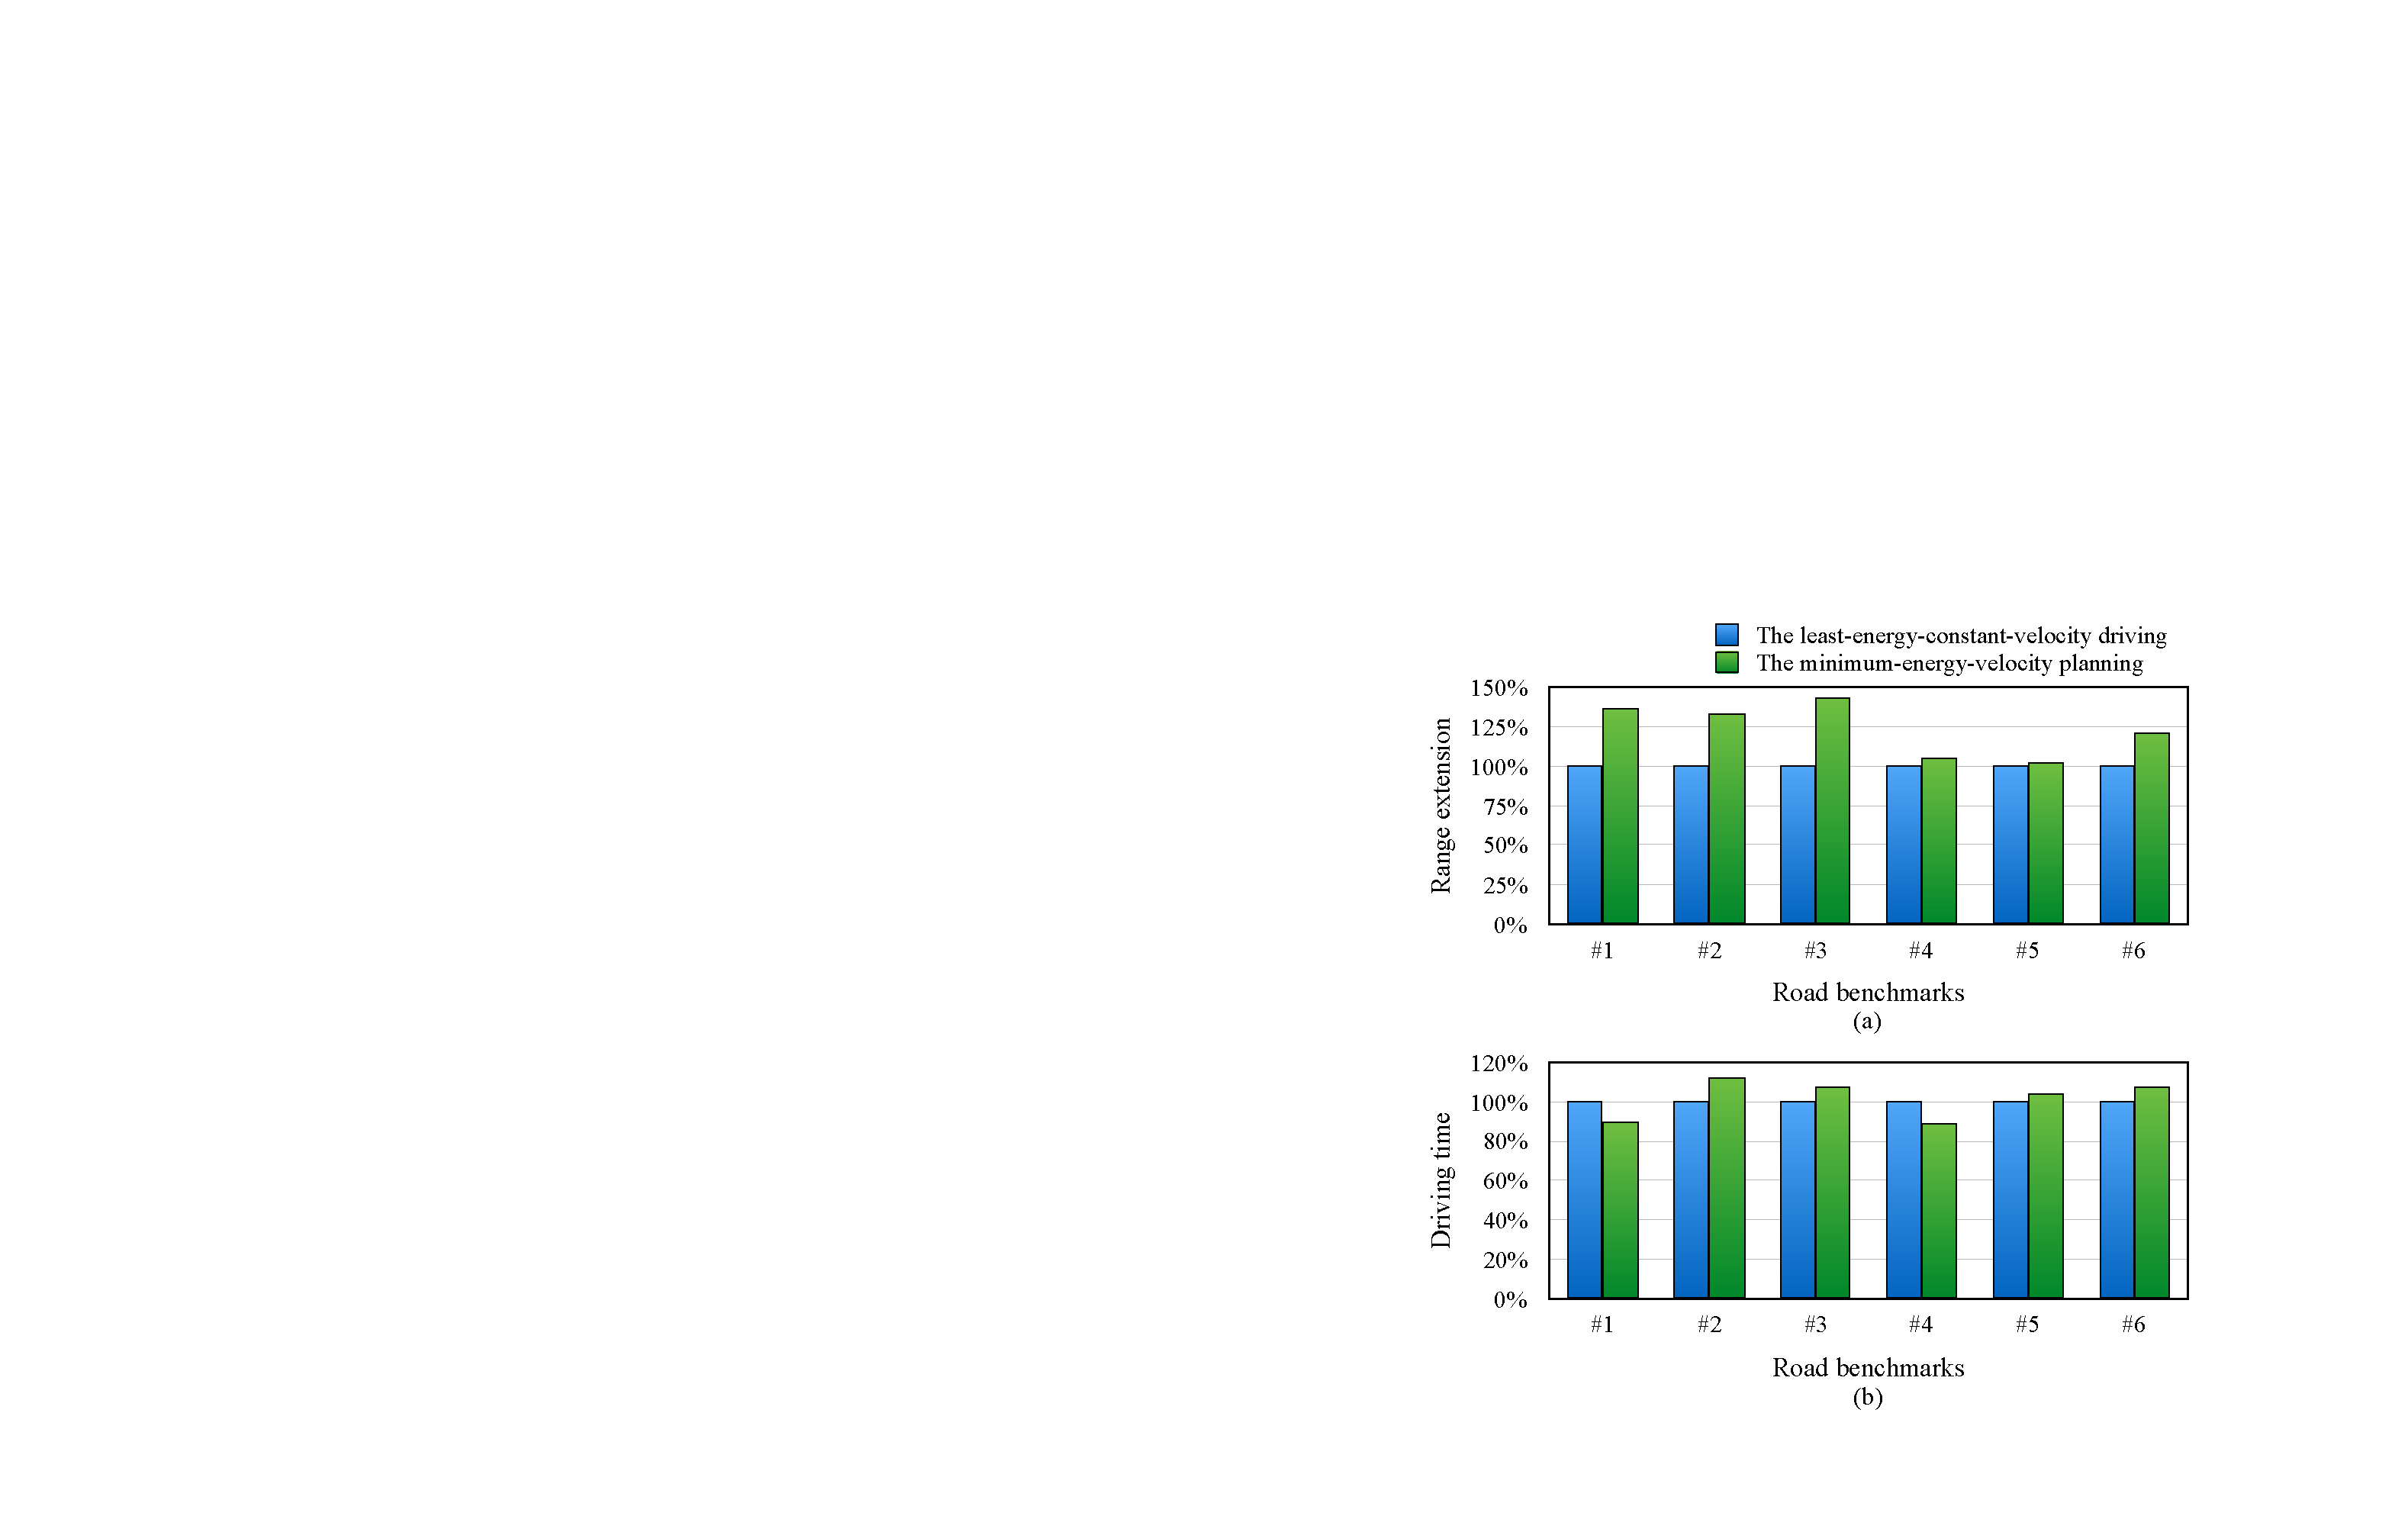
\includegraphics[width=1.0\hsize]{Figures/no_deadline_bar.pdf}
\caption{Range and time saving by the minimum-energy-velocity planning.}
\label{fig:no_deadline_bar}
\end{figure} 


\begin{figure} 	%Figure 9
\centering
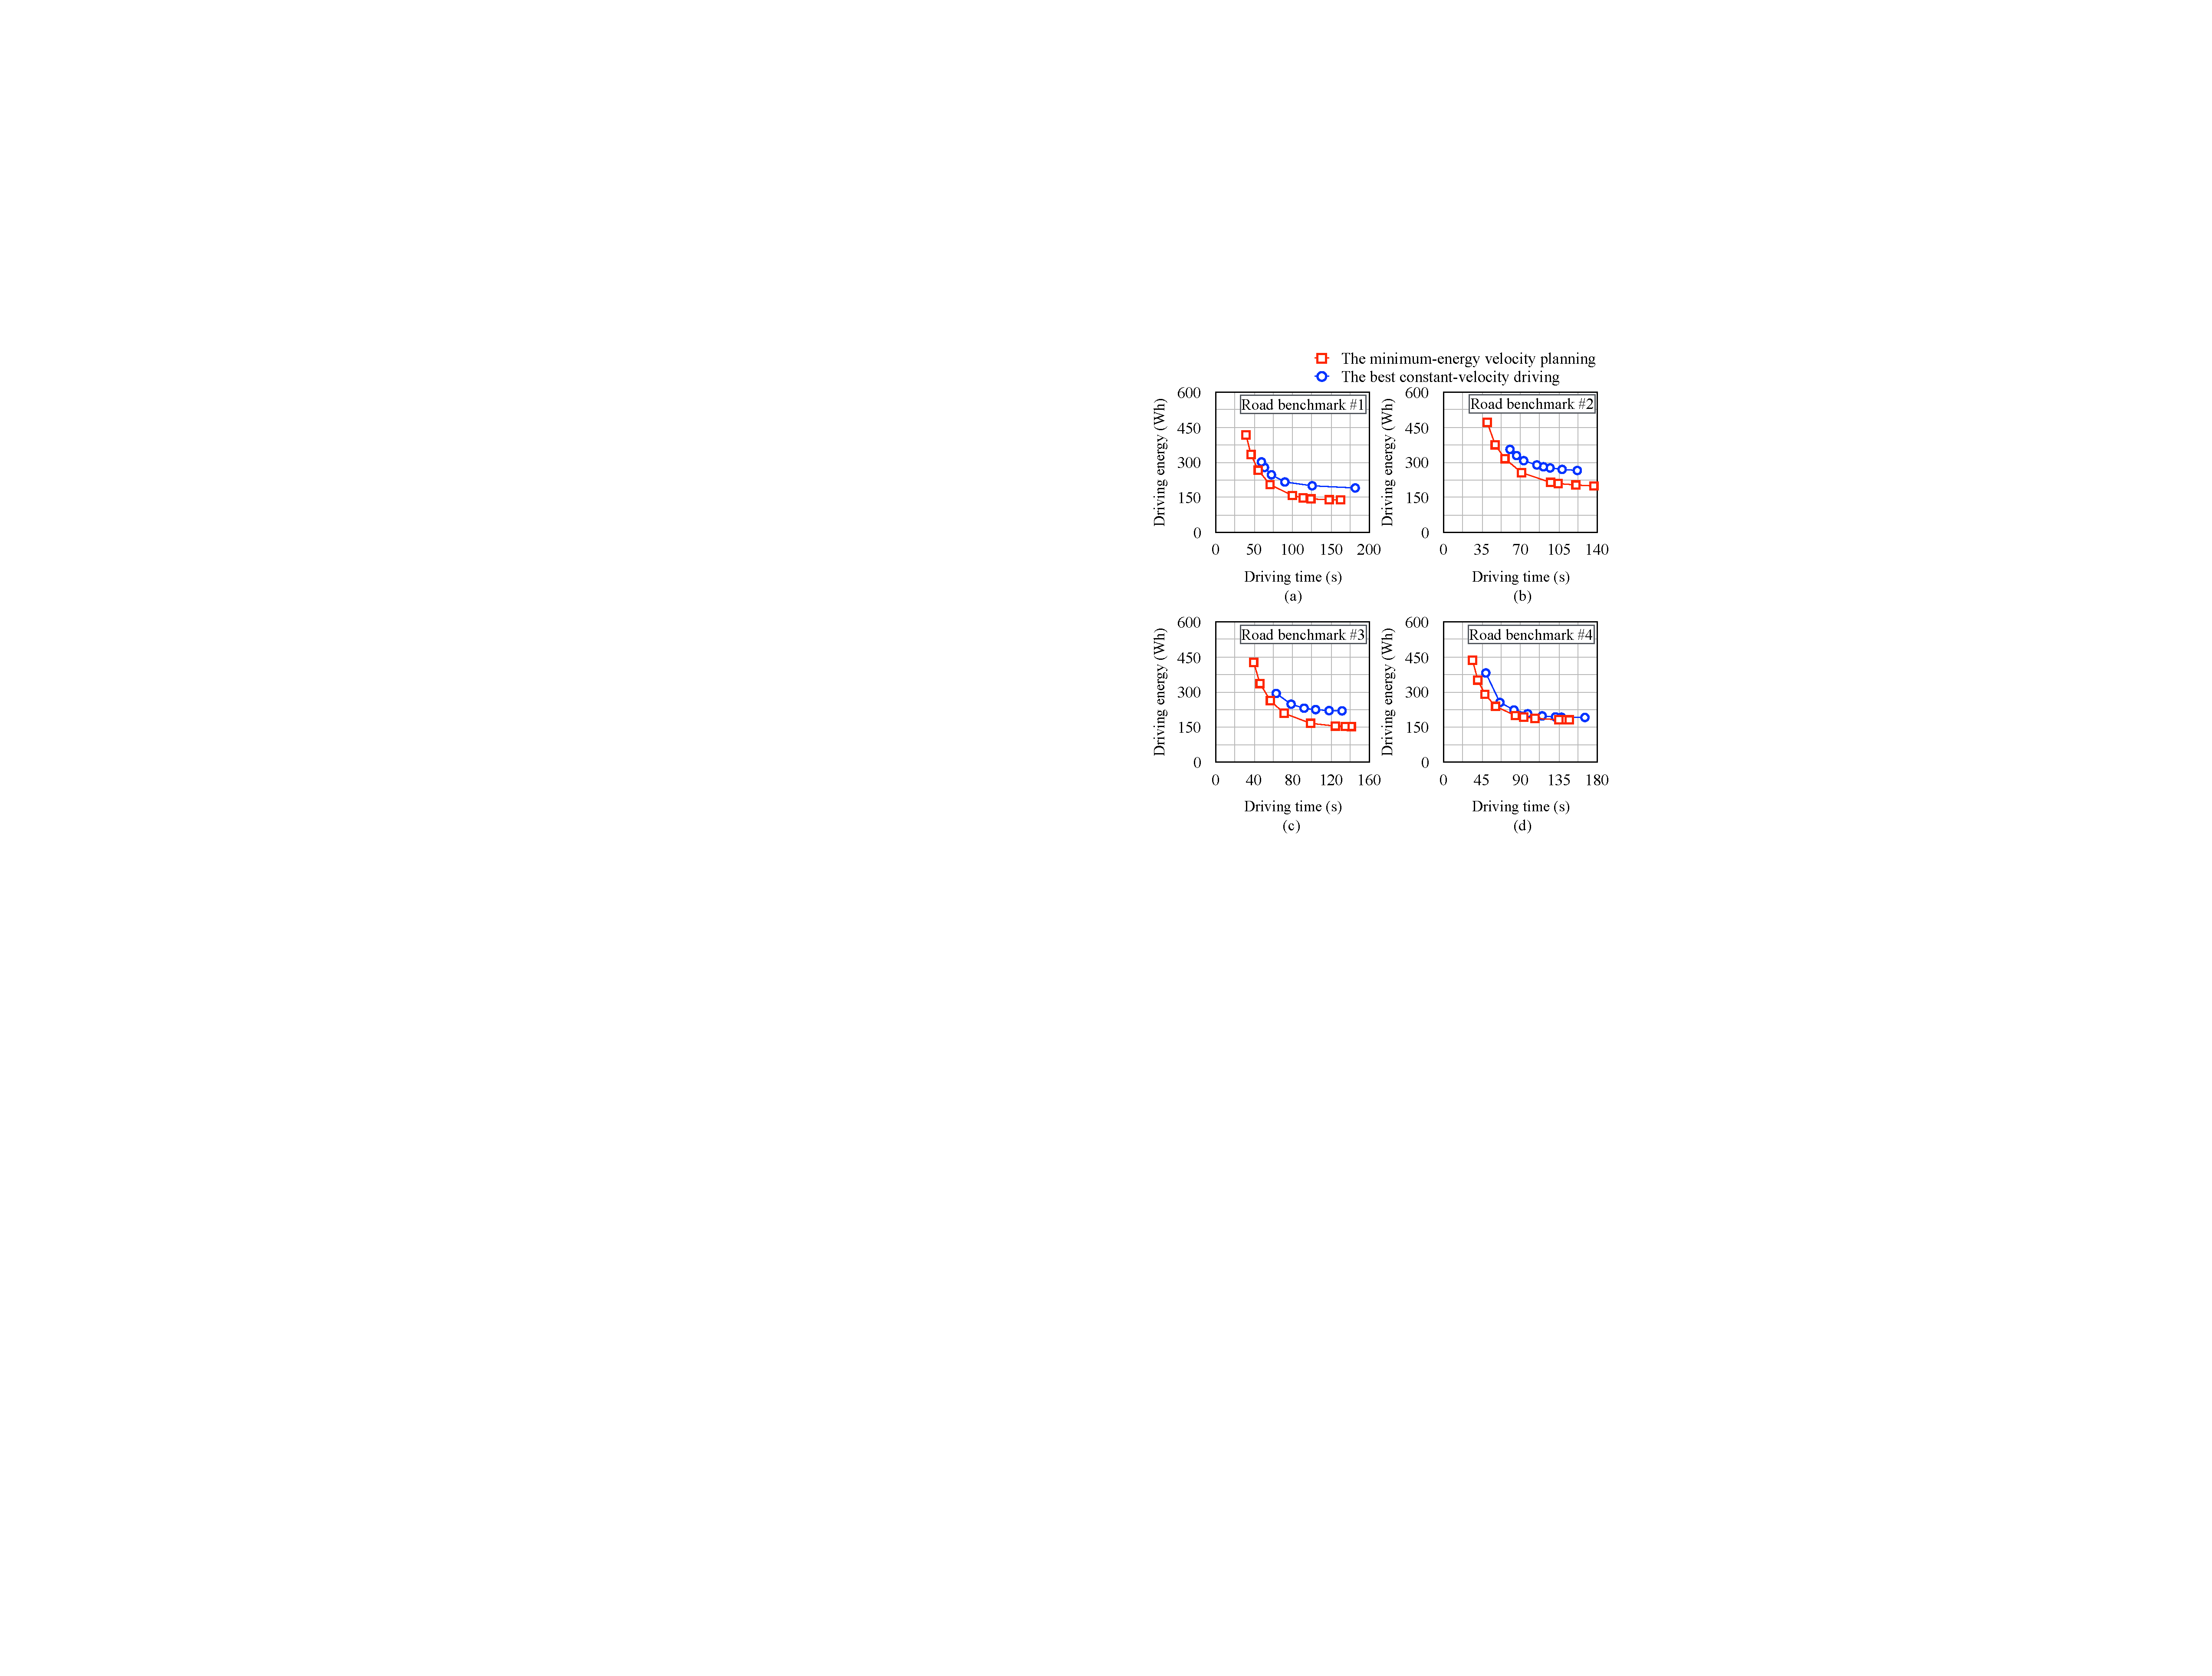
\includegraphics[width=\hsize]{Figures/ED_curve.pdf}
\caption{Energy-delay curves in road benchmarks.}
\label{fig:energy_delay_curve}
\end{figure} 

\begin{figure*} %Figure 10
\centering
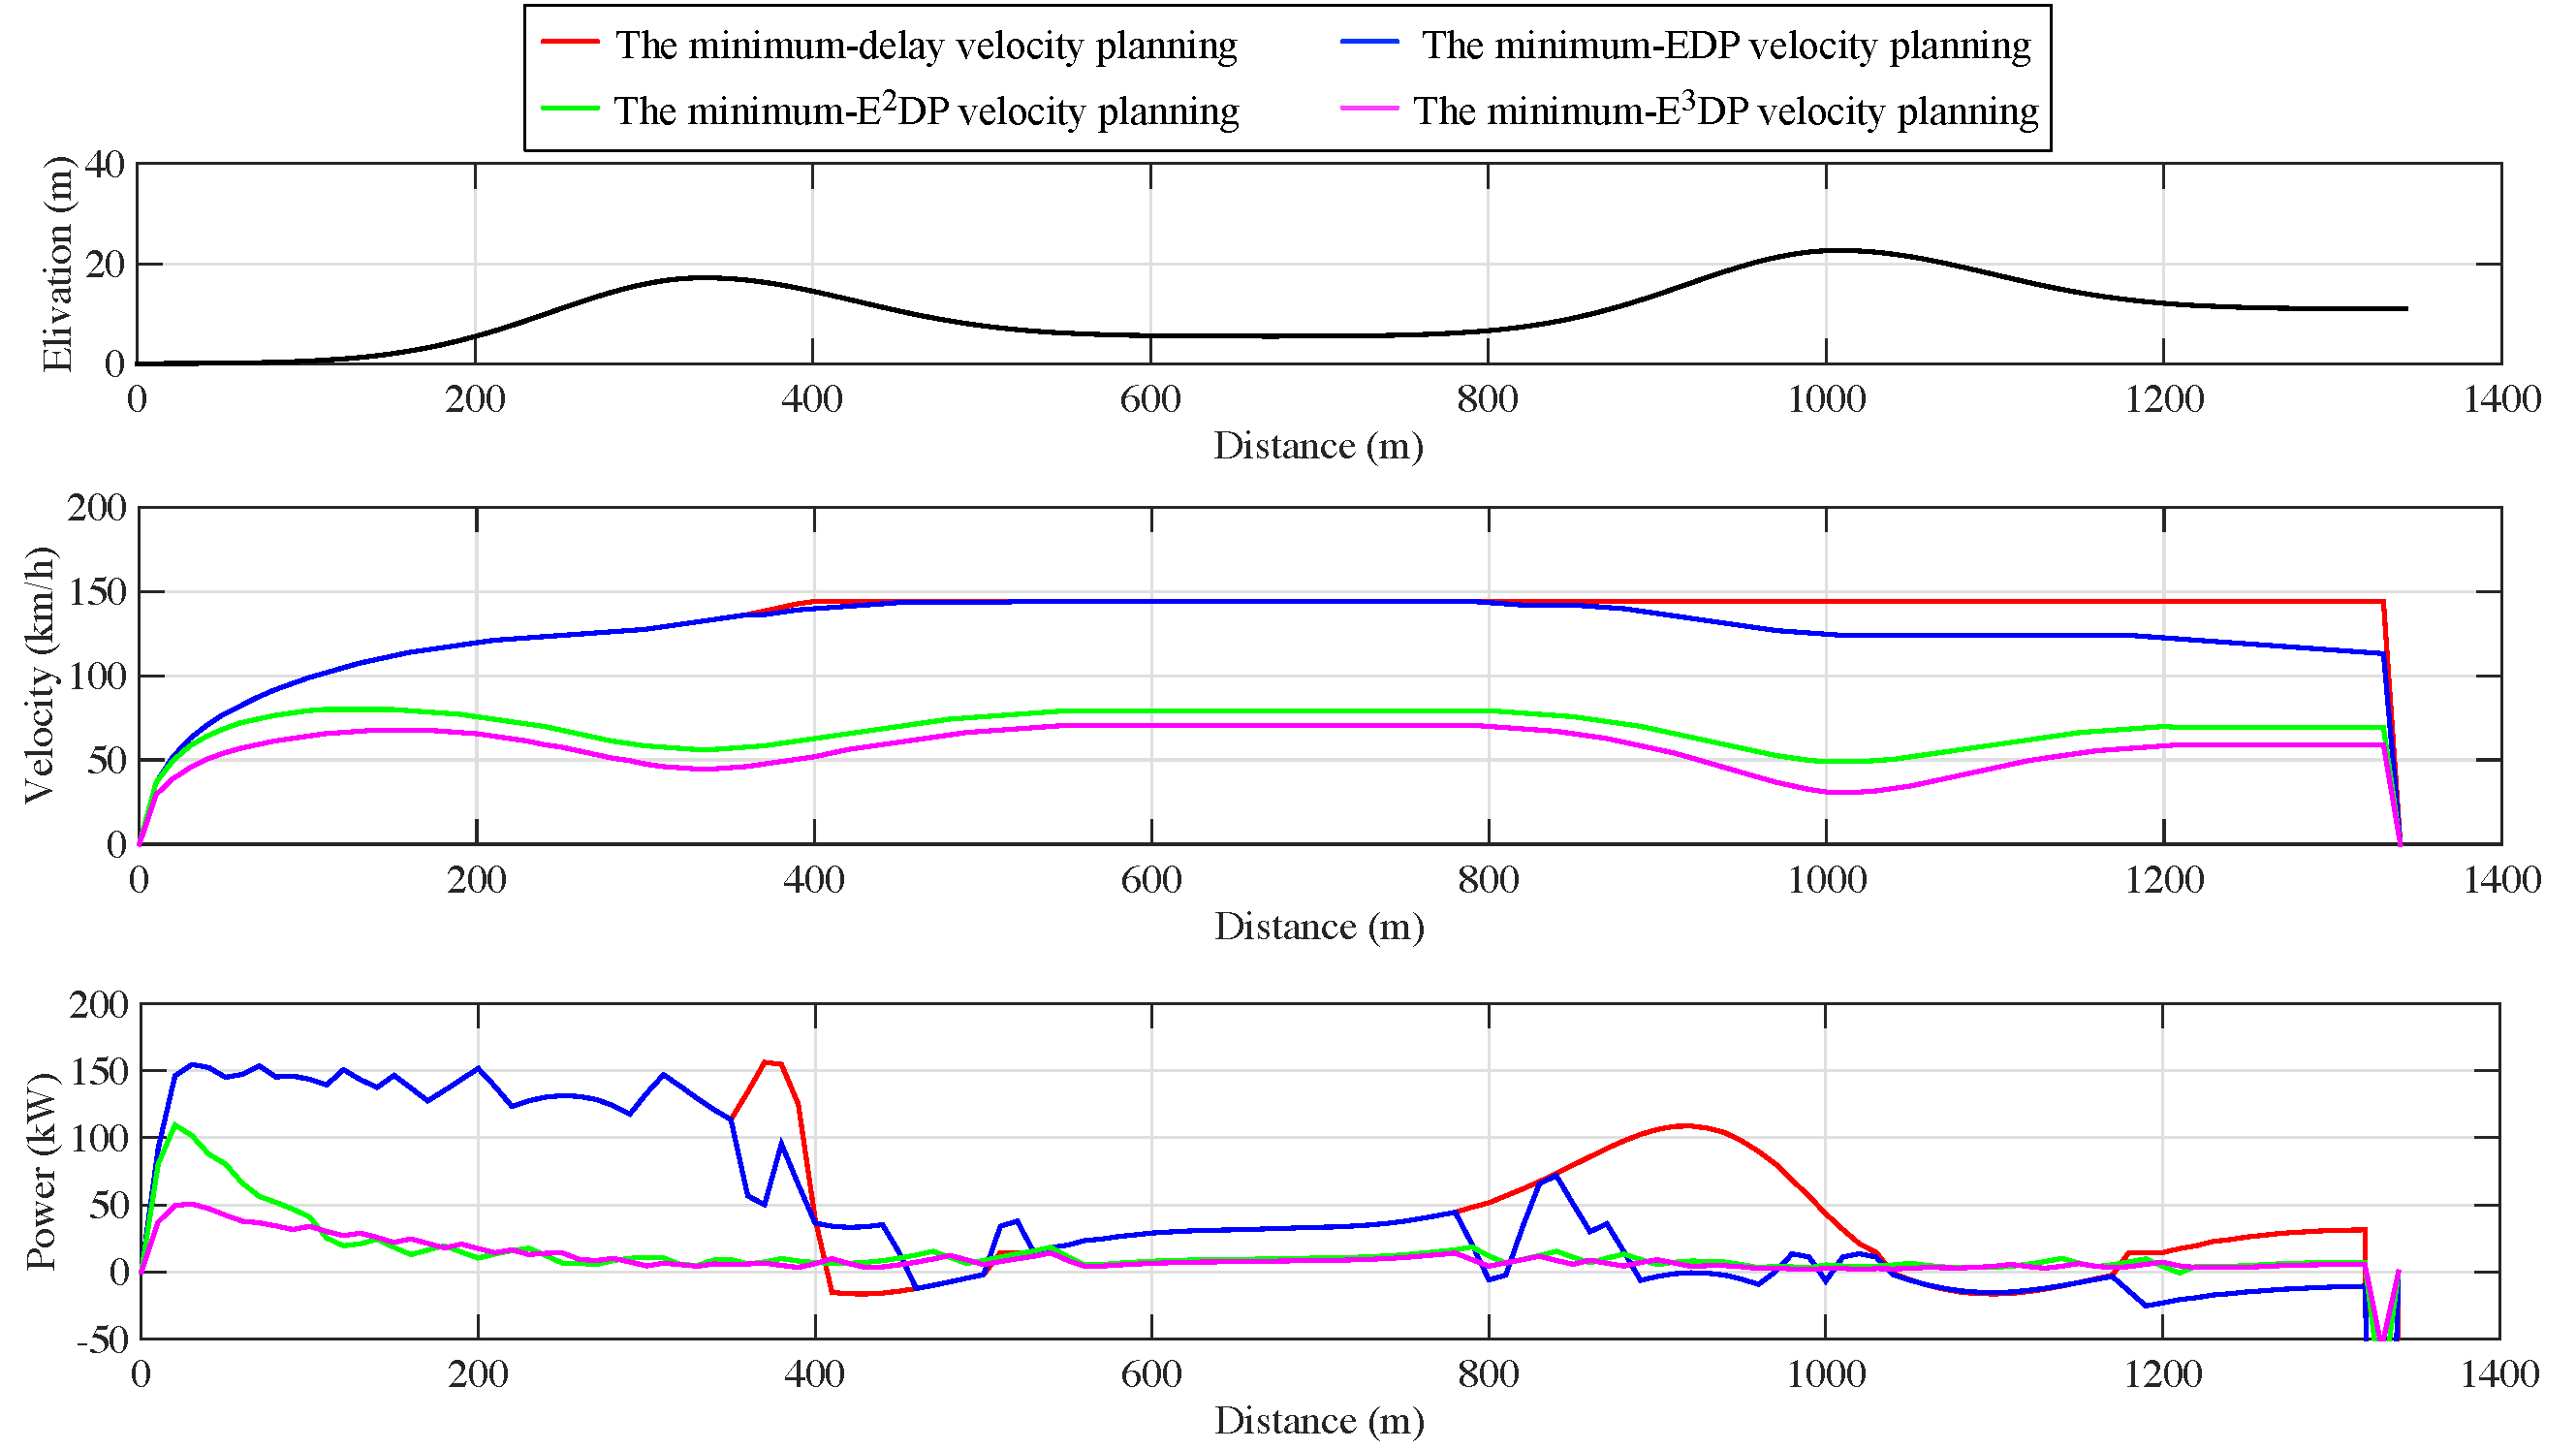
\includegraphics[width=1.0\hsize]{Figures/EDP_velocity_planning.pdf}
\caption{Velocity profile comparison with optimization of delay, $EDP$, $E^2DP$, and $E^3DP$.}
\label{fig:EDP_aware_velocity_planning}
\end{figure*} 


The energy-delay curves show the merit of the proposed velocity planning compared with the best constant-velocity driving with a deadline. We plot the relationship between driving energy and driving time with deadline constraints in Fig.~\ref{fig:energy_delay_curve}. X-axis and y-axis denote the EV driving time and energy under given deadlines, respectively. The energy-delay plot is useful to figure out the Pareto optimal velocity profiles. The energy-delay curves of the minimum-energy-velocity planning are located under the best constant-velocity driving curves, which implies that the minimum-energy-velocity planning is better than that of the best constant-velocity driving in terms of energy consumption under the same deadline. The same is true for the driving time under the same energy budget.

However, it is hard to compromise energy and driving time in general. In this paper, we propose to use energy-delay product ($EDP$), energy-square-delay product ($E^2DP$), or energy-cubic-delay product ($E^3DP$) so that a single metric can consider both energy and driving time. 
%
DP is a method for solving a complex problem by breaking it down into a collection of simpler subproblems, solving each of those subproblems just once, and storing their solutions. This enables the DP solve a complex problem in a polynomial time. DP solves the minimum-energy-velocity planning such that the minimum energy from interval $[0,\cdots,n]$ (the entire path) is divided into a partial problem of finding the minimum-energy-velocity planning for the interval of $[0, \cdots, i]$ and that for the interval of  $[i+1, \cdots, n]$:
%
\begin{align}
 (\Delta t_0 P_0 + \Delta t_1 P_1 + \cdots + \Delta t_n P_n)
 = (\Delta t_0 P_0 + \Delta t_1 P_1 + \cdots + \Delta t_i P_i) \nonumber \\
 + (\Delta t_{i+1} P_{i+1} + \cdots + \Delta t_n P_n). \nonumber
\end{align}

However, the minimum-EDP velocity planning problem cannot be divided into partial problems. In other words, the minimum-EDP velocity planning for the interval of $[0, \cdots, n]$ cannot be divided into a subproblem for the interval of $[0, \cdots,  i]$ and that for the interval of $[i+1,\cdots, n]$.
%
\begin{align}
&(\Delta t_0 P_0 + \Delta t_1 P_1 + \cdots + \Delta t_n P_n)(\Delta t_0 + \Delta t_1 + \cdots + \Delta t_n) \nonumber \\ 
&\neq (\Delta t_0 P_0 + \Delta t_1 P_1 + \cdots + \Delta t_i P_i)(\Delta t_0 + \Delta t_1 + \cdots + \Delta t_i) \nonumber \\
&+ (\Delta t_{i+1} P_{i+1} + \cdots + \Delta t_n P_n)(\Delta t_{i+1} + \cdots + \Delta t_n). \nonumber
\end{align} 

The same is true for the minimum-$E^2DP$ or $E^3DP$ velocity planing problem as well. Therefore, in this paper, we propose a heuristics method that still uses DP for the minimum-$EDP$, $E^2DP$ and $E^3DP$ velocity planning. The heuristics does not explicitly optimize $EDP$, $E^2DP$ or $E^3DP$ but still take into account the awareness of them by the use of $EDP$, $E^2DP$ or $E^3DP$ as a cost function. 

Figure~\ref{fig:EDP_aware_velocity_planning} shows the EDP-aware velocity planning. 
If energy-delay product ($EDP$) is used as a cost function, the optimization considers both energy and delay penalty. However, the $EDP$-aware velocity planning often overrides the minimum-energy-velocity because the delay penalty due to the reduced velocity is greater than the energy penalty due to the increased torque. Therefore, this policy can be used when the deadline is tight. Chances of energy saving by the minimum-energy-velocity planning decrease as the deadline becomes tighter. 
The velocity planning attempts to reduce driving time with a constant velocity rather than deceleration at the top of the hill. 
%
The $EDP$-aware velocity planning similarly accelerates to the minimum-energy-velocity (or the minimum velocity constraint, whichever comes first) by the road slope. However, the planning does not decelerate at the top of the hill to reduce driving time. It only slightly slows down when climbing up an uphill at the maximum velocity since the energy penalty become higher than the delay penalty. The EV keeps driving at the same velocity on the downhill and the following float road until it arrives at the destination. So, if the deadline is tight, we use $EDP$ for the metric.

On the other hand, when the square of energy-delay product ($E^2DP$) is used as a metric to optimize, the energy penalty contributes more to the cost function. As a result, the driving velocity decreases when driving on an uphill because the energy penalty due to the increased torque is greater than the delay penalty as shown in Figure~\ref{fig:EDP_aware_velocity_planning}. Also, the $E^2DP$-aware vehicle velocity becomes slower than the maximum velocity on a downhill or on a flat road since the energy penalty becomes higher than the delay penalty at a high velocity due to the drivetrain loss and increased torque by the aerodynamic resistance. The EV accelerates to the minimum-energy-velocity (or the minimum velocity constraint, whichever comes first) by the road slope and decelerates at the top of the first hill. Then, the EV drives faster than the minimum-energy velocity on the downhill followed by a  flat road, in preparation for the next hill. Although the minimum-energy velocity on an uphill is higher than that on a flat road, climbing an uphill consumes more energy. So, the EV gradually loses the velocity while it climbs up on an uphill spending less motor torque, which significantly saves energy consumption. In most applications, the deadline is important but not hard. Therefore, we adopt $E^2DP$ for the performance metric to consider both energy and driving time.
%The EV applies regenerative braking on the downhill and drives at the minimum-energy velocity on the following flat road until it arrives at the destination.

When it comes to energy-cubic-delay product ($E^3DP$), the effect of energy penalty becomes even more distinct, the average driving velocity becomes lower, and the energy consumption is reduced thanks to regenerative braking. The $E^3DP$ metric can be a proper optimization metric when the battery state of charge is less than 30\% for example.

Figure~\ref{fig:EDP_bar} shows energy-delay product of the best constant-velocity driving and the velocity planning with $EDP$, $E^2DP$ and $E^3DP$ as a metric on the five road benchmarks. The leftmost bars indicate the best constant-velocity driving, which minimizes the energy-delay product. The proposed velocity planning results in average 9.9\% and up to 20.6\% improvements of energy-delay product. The improvements occur especially when the slope of the uphill is steep. The driving velocity on a flat road is faster than that of the best constant-velocity driving at the expense of relatively little energy to save driving time. Then, the velocity decreases when climbing the following uphill to spends less motor torque, which saves more energy.

\begin{figure}	 %Figure 11.
\centering
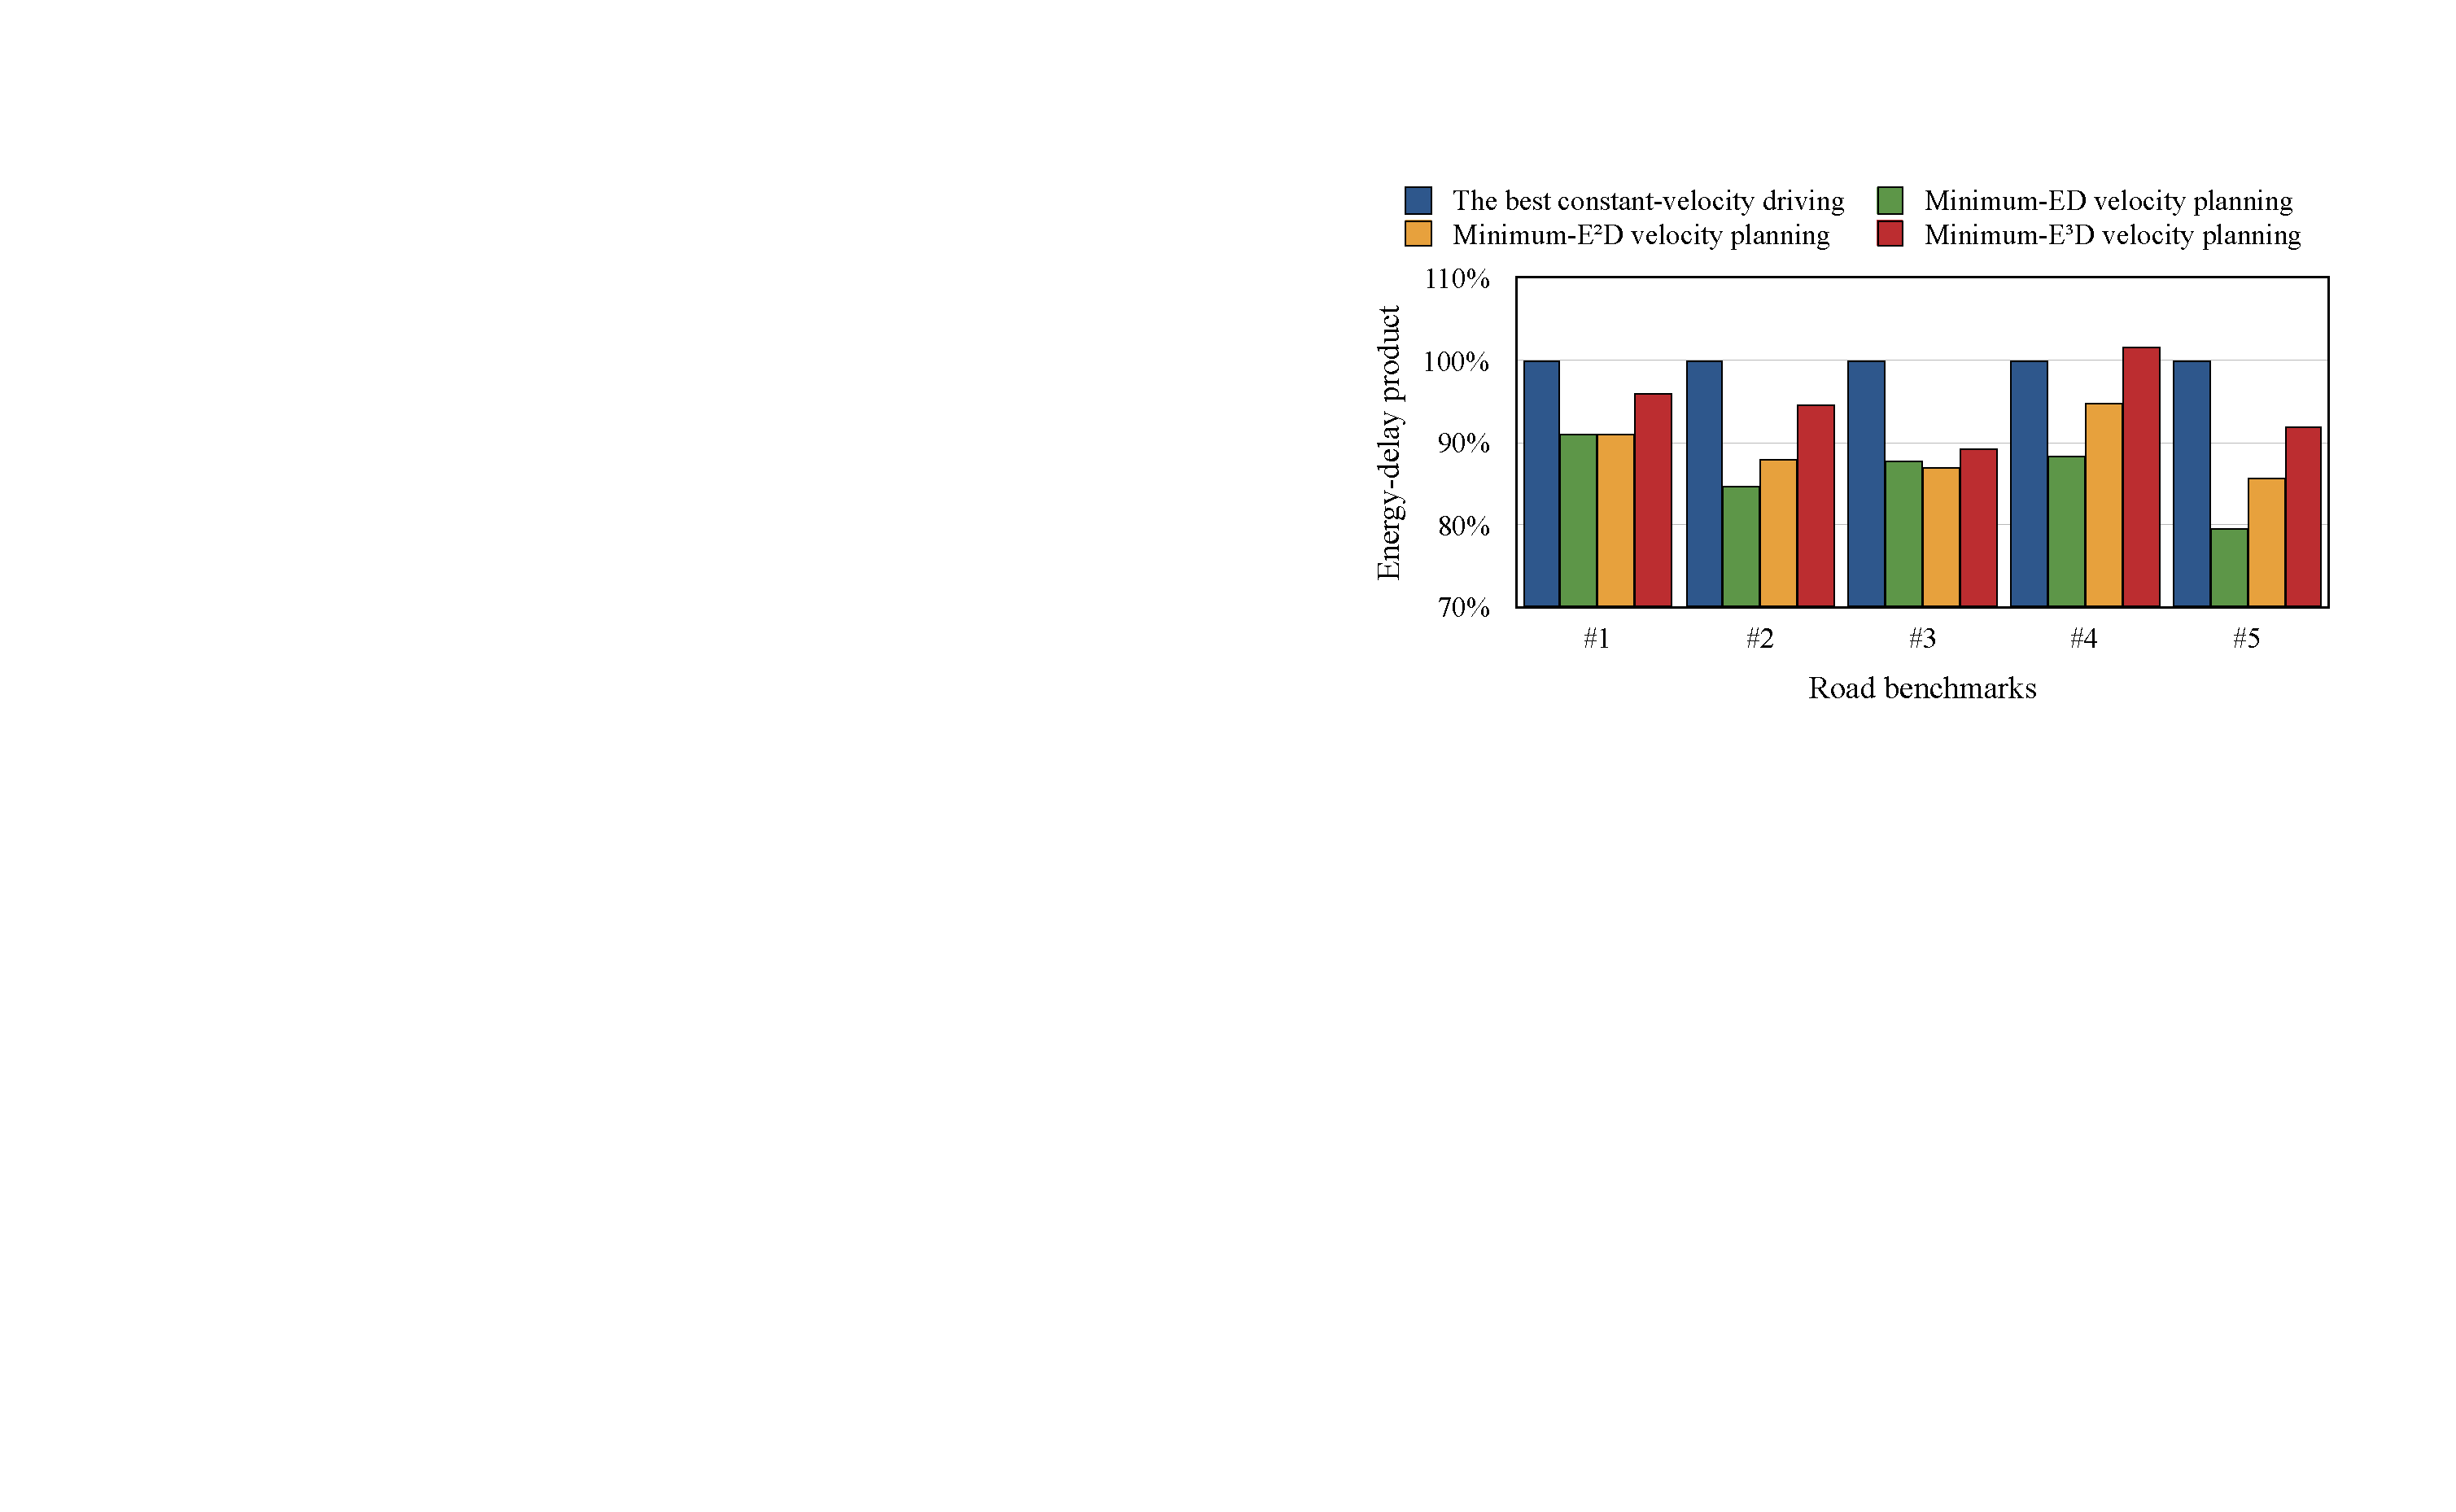
\includegraphics[width=\hsize]{Figures/EDP_bar.pdf}
\caption{Energy-delay product comparison.}
\label{fig:EDP_bar}
\end{figure} 


%%%%%%%%%%%%%%%%%%%%%%%%%%%%%%%%%%%%%%%%%%
\section{Impact of the EV power model fidelity} \label{sec:impact_EV_power model}
%%%%%%%%%%%%%%%%%%%%%%%%%%%%%%%%%%%%%%%%%%

Lesson learned from embedded systems power management, it is crucial to extract an accurate power model from the device to system. Power optimization results largely change by the power model. Inaccurate power model obviously misleads the power optimization results. It goes without saying that an accurate EV power model mandates for the minimum energy velocity problem that reflects power variation by the velocity, acceleration, road slope, payload, and so forth.

\begin{figure}	 %Figure 12.
\centering
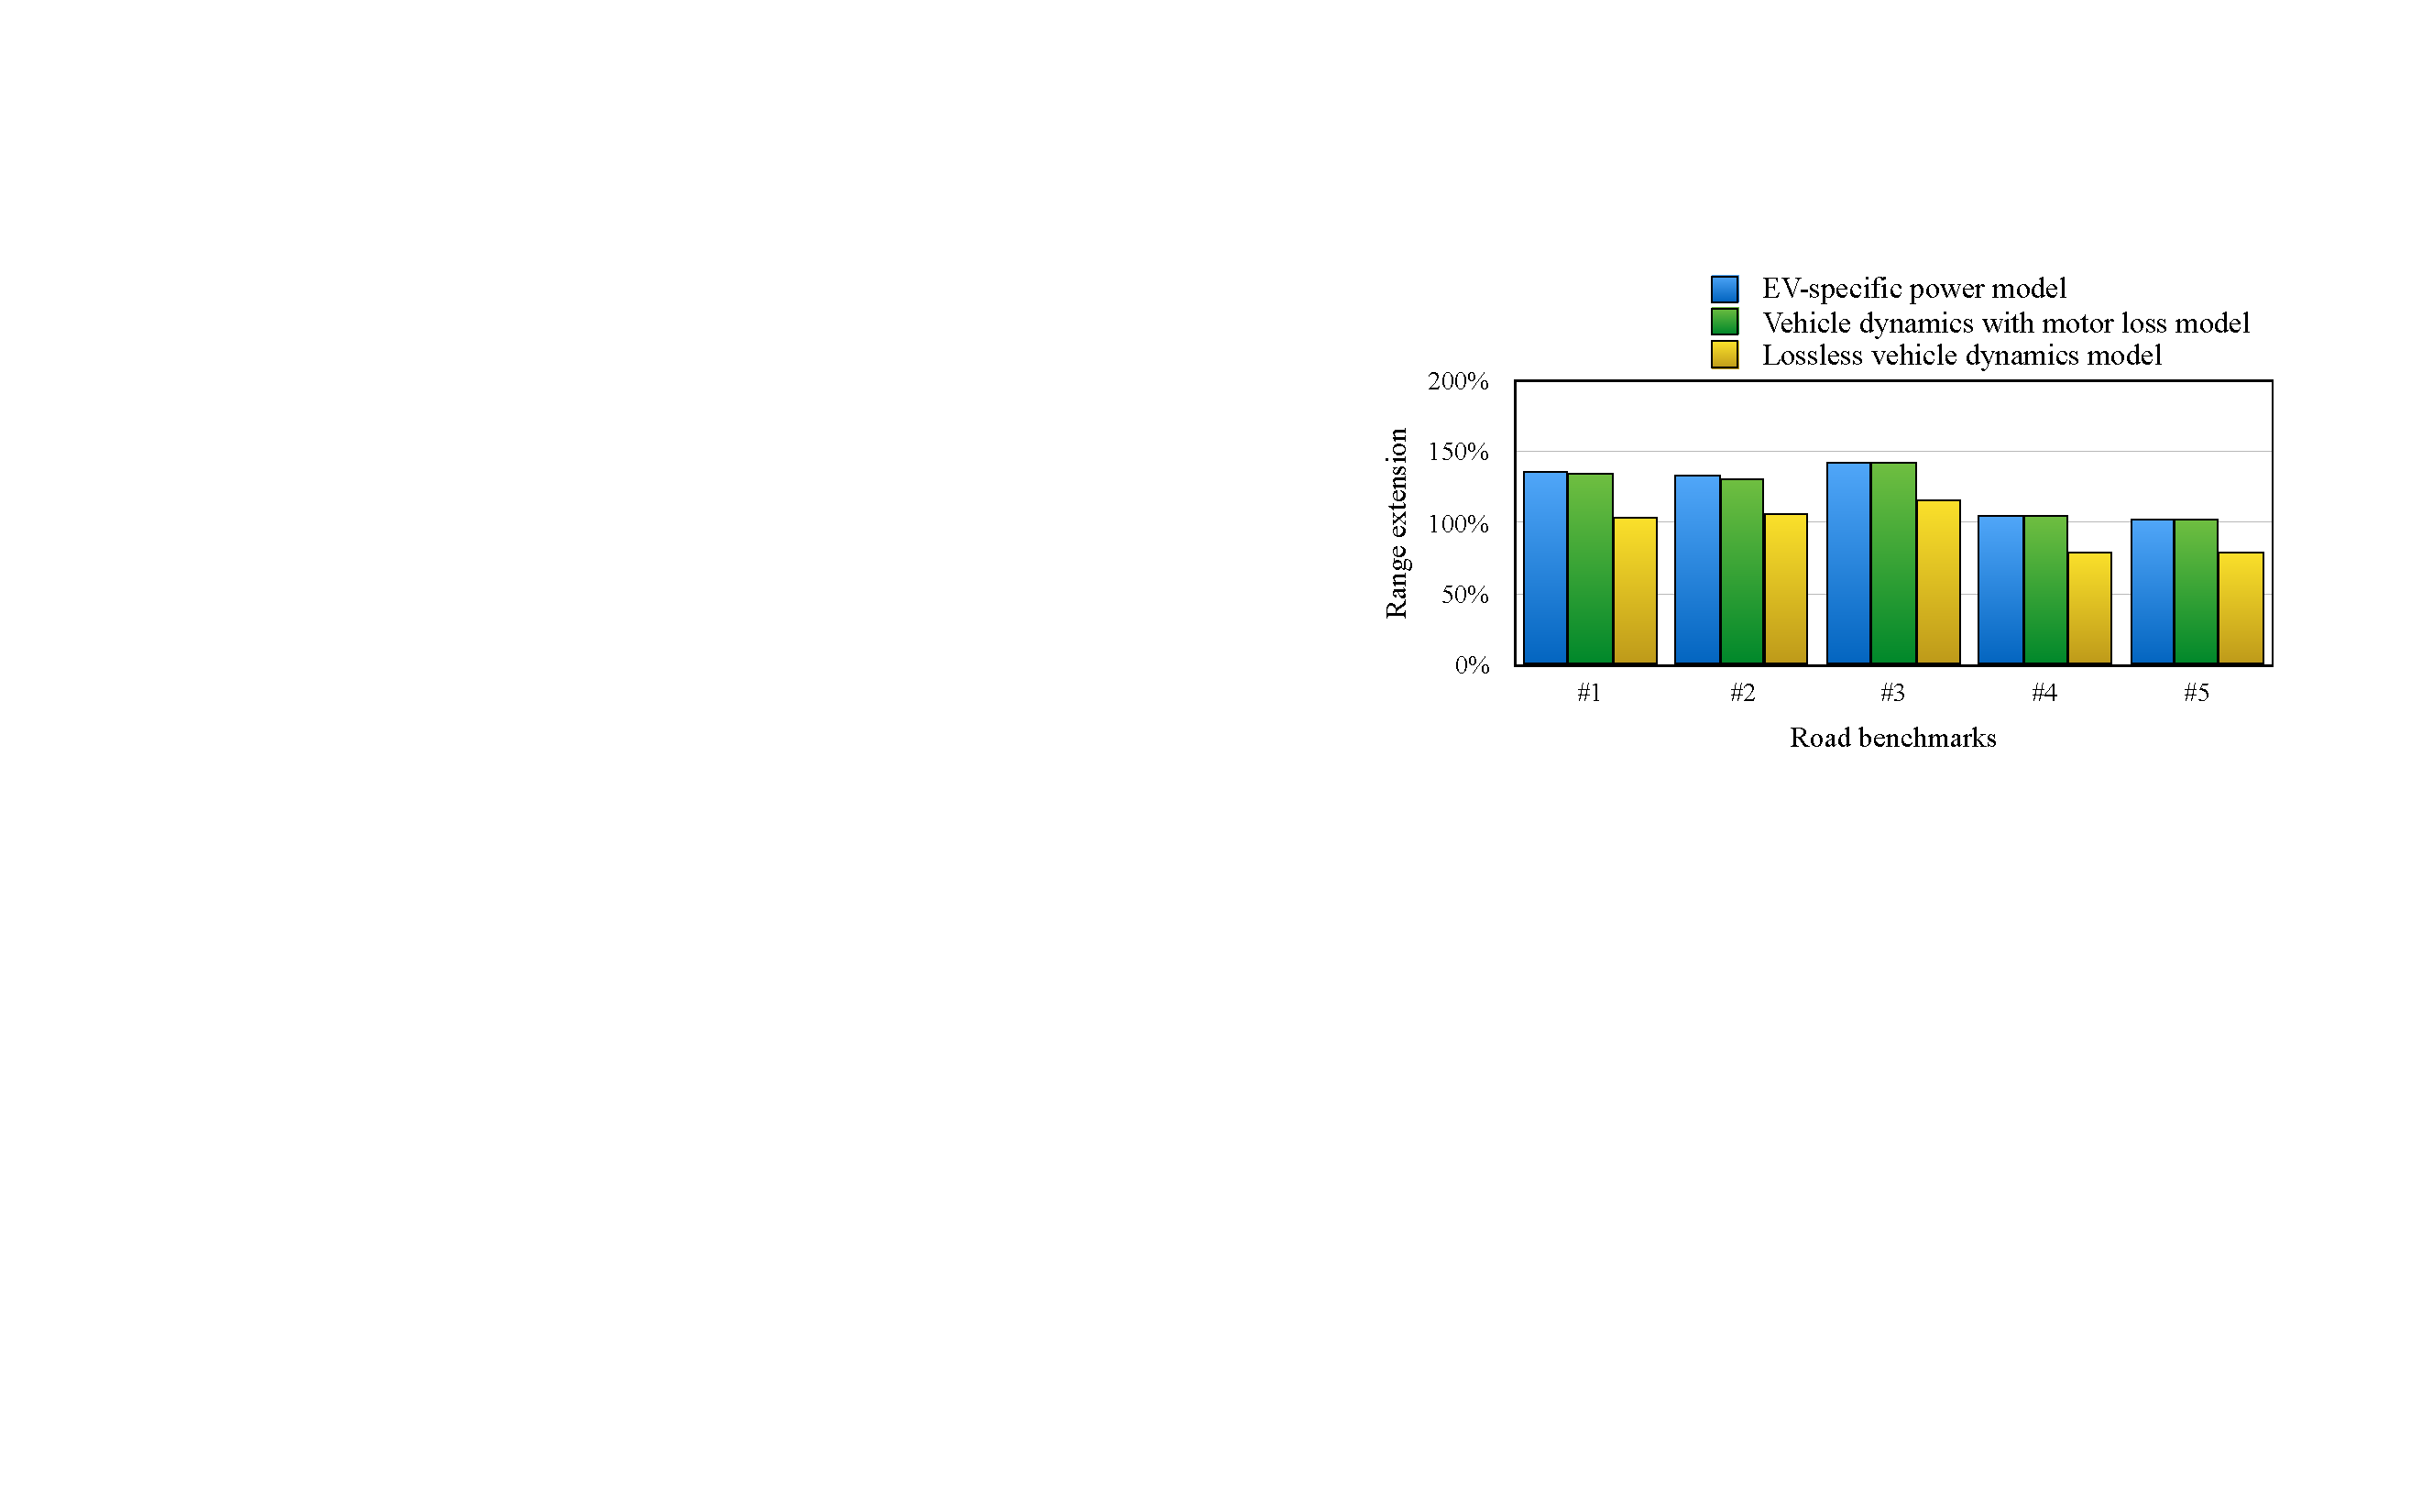
\includegraphics[width=\hsize]{Figures/model_fidelity.pdf}
\caption{Range comparison by EV power consumption models.}
\label{fig:energy_by_model}
\end{figure} 

We compare the minimum-energy-velocity planning results with i) a lossless vehicle dynamics model (\ref{eq:dynamics_model}), ii) a vehicle dynamics model with motor loss (\ref{eq:motorloss_model}) and iii) an EV-specific power model (\ref{eq:EV_specific_model}) described in Section~\ref{subsec:opt-cruising}. Inaccurate EV power consumption model causes suboptimal EV driving optimization.

Figure~\ref{fig:energy_by_model} shows the comparison of range extension by the EV power models. The X-axis indicates the types of benchmark road slopes, and y-axis indicates the range; 100\%  range implies the range by the best constant-velocity driving. Black bars indicate the range with the lossless vehicle dynamics model, which does not consider motor loss and vehicle power loss at the drivetrain. White and gray bars indicate the range with the vehicle dynamics with motor loss model and the EV-specific power model, respectively.

Driving optimization using more accurate power model shows more extended range. The extended range with the EV-specific power model is average 1.6\% and 32.8\% compared with the minimum-energy-velocity planning with the vehicle dynamics with motor loss model and lossless vehicle dynamics model, respectively. One of main reasons is that the underestimated EV power loss becomes a considerable portion of total energy consumption when the EV drives on low road slope or downhill.

%%%%%%%%%%%%%%%%%%%%%%%%%%%%%%%%%%%%%%%%%%
\section{Conclusions} \label{sec:conclusions}
%%%%%%%%%%%%%%%%%%%%%%%%%%%%%%%%%%%%%%%%%%

This paper introduces a novel minimum-energy-velocity planning for all-electric vehicles (battery electric vehicles, BEV), which is inspired by low-power scheduling for computing systems. This work is a showcase such that legacy system-level  low-power design methodologies significantly improves electric vehicle fuel efficiency. We demonstrate the potential gain from the proposed minimum-energy-velocity planning for EV. We show the importance of EV-specific power model  comparing the actual energy gain from EV using different fidelity power models. In addition, this paper is the first to show the difference of the minimum-energy-velocity planning between the full electric vehicles and internal combustion engine vehicles. Most importantly, we introduce energy and time combined metrics such as, energy-delay product ($EDP$), energy-square-delay product ($E^2DP$) and energy-cubic-delay product ($E^3DP$) for a tight time deadline constraint, a lose time deadline constraint, and a tight deadline constraint, respectively. 
The proposed method results in up to a 43.4\% extended range and a  20.6\% improvement of the energy-delay product compared with the best constant-velocity driving. 
The minimum-energy-velocity planning will become more crucial when full autonomous driving is widely deployed.


%%%%%%%%%%%%%%%%%%%%%%%%%%%%%%%%%%%%%%%%%%%
%\section*{Acknowledgment}
%%%%%%%%%%%%%%%%%%%%%%%%%%%%%%%%%%%%%%%%%%%
%
%This work was supported by the National Research Foundation of Korea (NRF) grant funded by the Korea government (MSIP) (No. 2015R1A2A1A09005694.)

\bibliographystyle{ieeetr}
\bibliography{EV}

% that's all folks
\end{document}
